%!TEX root = ../main.tex

%\begin{itemize}
% 
%  \item 2.1 - describe the jsil language. give its formal syntax  and semantics (extended with assert). 
%                   formally define symbolic execution for JSIL commands. soundness result and its corollaries.  
% 
%  \item 2.2 Implementation:  
%               - describe the \rosette approach to the implementation of symbolic analysis 
%               - describe the encoding of \jsil concrete/symbolic states in \rosette 
%               - explain the \jsil interpreter implemented in \rosette and its connection to the \jsil concrete semantics  and symbolic semantics 
%               		- give snippets of the interpreter 
%	       		- discuss implementation strategies that enable \rosette to work properly
%\end{itemize}

We introduce our symbolic execution engine for \jsil~\cite{javert}. In~\S\ref{subsec:jsil:analysis:formalism}, we present 
the theoretical underpinnings of the symbolic analysis, whereas, in \S\ref{subsec:jsil:analysis:implementation}, 
we describe its implementation in \rosette~\cite{Rosette1,Rosette2}.

\vspace*{-0.2cm}
\subsection{Formalisation}\label{subsec:jsil:analysis:formalism}

\vspace*{-0.2cm}
\myparagraph{\jsil: Syntax} \jsil is a goto language featuring top-level procedures and commands operating on object heaps. It was purposefully designed to natively support the main dynamic features of JavaScript: extensible objects; dynamic property access; and dynamic procedure calls. 

\jsil \emph{values}, $\val \in \vals$, include numbers, booleans, strings, the special values $\jsundefined$ and $\jsnull$, as well as types~$\ivltype$, procedure identifiers $\fid$, and the special value $\jsilempty$. 
\jsil~\emph{expressions}, $\jsilexpr \in \exprs$, include \jsil values, \jsil program variables $\jvar$, and various unary and binary operators, which, for instance, provide support for sets and lists. 


%\pg{When talking about JSIL Logic, how are you going to explain the difficulty associated with a dynamci goto language v a static one, I don't think your work is a boring adaptation of reasoning about a staitc goto language. You need to grab at some of this is you can. We've have not paid ebough attention on this, so people jsut think this is a variant of previous work..} 

\begin{figure}[!t]
\begin{minipage}{\textwidth}
\begin{tabular}{lllll}
	 Numbers: $\jnumber \in \numbers$ &  Booleans: $\jbool \in \bools$ & \  \ Strings: $\jstring \in \strings$ & \  \ Locs: $\loc \in \locs$ & \  Vars: $\jvar \in \jvars$ \\[0.1cm]
	Types: $\ivltype \in \ivltypes$ & \multicolumn{4}{l}{Values: $\val \in \vals$ \defeq \ $\jnumber \mid \jbool \mid \jstring \mid  \jsundefined \mid \jsnull \mid \loc \mid \ivltype \mid \fid \mid \jsilempty$} \\[0.1cm]
\multicolumn{5}{l}{Expressions: $\jsilexpr \in \exprs$ \defeq \ $\val \mid \jvar \mid \ominus\ \jsilexpr \mid \jsilexpr \binop{} \jsilexpr $} \\[0.1cm]
	\multicolumn{5}{l}{Basic Commands: $\bcmd \in \bcmds$ \defeq\ $\jsilskip \mid \jvar := \jsilexpr  \mid \jvar := \jsilnew() \mid \jvar := [\jsilexpr, \jsilexpr] \mid [\jsilexpr, \jsilexpr] := \jsilexpr \mid$} \\[0.1cm]
	\multicolumn{5}{l}{\hspace{2.8cm} $\jsildelete(\jsilexpr, \jsilexpr) \mid \jvar := \hasfield(\jsilexpr, \jsilexpr) \mid \jvar := \getfields(\jsilexpr) \mid \assume(\jsilexpr) \mid \assert(\jsilexpr)$} \\[0.1cm]
	% Commands
	\multicolumn{5}{l}{Commands: $\ivlcmd \in \cmds$ \defeq \ $ \bcmd \mid \goto \ i \mid  \ifgoto{\jsilexpr}{i}{j} \mid \jsilcall{\jvar}{\jsilexpr}{\jvec{\jsilexpr}}{j}$} \\[0.1cm]
	\multicolumn{5}{l}{Procedures : $\proc \in \procset$ \defeq \ $\procedure{\fid}{\jvec{\jvar}}{\jvec{\ivlcmd}}$}
 \end{tabular}
 \vspace*{-0.2cm}
 \caption{Syntax of the \jsil Language}
 \label{def:jsil-types}
 \end{minipage}
  \vspace*{-0.5cm}
 \end{figure}
 
%Most syntactic constructs of JSIL either come directly from JavaScript or are useful for JavaScript analysis. 


\jsil \emph{basic commands} enable the management of extensible objects and do not affect control flow. 
They include $\jsilskip$, variable assignment, object creation, property access, property assignment, property deletion, membership check, property collection, and two special commands, $\assume$ and $\assert$, essential for symbolic execution, but with trivial concrete semantics.
%
\jsil \emph{commands} include \jsil basic commands and several commands related to control flow: conditional gotos, unconditional gotos and dynamic procedure calls.\footnote{\jsil also has a $\phi$-node assignment, which allows \JSComp to produce code directly in Static-Single-Assignment (SSA) \cite{SSA}. To avoid clutter, we omit the $\phi$-node assignment from this formalisation as they do not impact the reasoning in any way. Details can be found in \cite{javert}.} 
The two goto commands are straightforward: $\goto \ i$ jumps to the $i$-th command of the active procedure, and $\ifgoto{\jsilexpr}{i}{j}$ jumps to the $i$-th command if $\jsilexpr$ evaluates to $\jtrue$, and to the $j$-th if it evaluates to $\jfalse$. 
The dynamic procedure call $\jsilcall{\jvar}{\jsilexpr}{\jvec{\jsilexpr}}{j}$ first evaluates  $\jsilexpr$ and $\jvec{\jsilexpr}$ to obtain the procedure name and arguments, respectively, executes the appropriate procedure with these arguments, and, in the end, assigns its return value to $\jvar$.
If the procedure raises an error, control is transferred to the $j$-th command, and to the next otherwise. 

A \jsil program $\prog \in \ivlprogs$ can be seen as a set of top-level procedures of the form $\procedure{\fid}{\jvec{\jvar}}{\jvec{\jcmd}}$, where $\fid$ is the procedure name, $\jvec{\jvar}$ its formal parameters, and its body ${\jvec{\jcmd}}$  is a \emph{command list} consisting of a sequence of \jsil commands.
Every \jsil program contains a special procedure $\jsilmain$\hspace{-2pt}, denoting the entry point of the program. 
\jsil procedures return via two dedicated indexes, $\procretlab$ and $\procerrlab$, using two dedicated variables, $\procretvar$ and $\procerrvar$. If a procedure reaches the $\procretlab$ index, it returns normally with the return value denoted by $\procretvar$; when it reaches $\procerrlab$, it returns an error, with the error value denoted by $\procerrvar$.

\myparagraph{\jsil: Semantics}
The basic memory model of \jsil is as follows. 
%\jsil values contain: numbers, $\jnumber$; booleans, $\jbool$; strings, $\jstring$;  the special values \jsinline|undefined| and \jsinline|null|; and object locations,  $\loc \in \locs$.
A \jsil heap, $\heap \in \heaps$, is a partial function mapping pairs of  object locations, and strings to heap values. 
 Given a heap $\heap$, we denote: a heap cell by $\hcell{\loc}{\jstring}{\val}$, meaning that  $h(\loc,\jstring) = \val$; the union of two disjoint heaps by $\oheap_1 \dunion \oheap_2$; heap lookup by $\hread{\oheap}{\loc}{\jstring}$; and the empty heap by $\hemp$.
 Finally, a \jsil variable store, $\store \in \stores$, is a mapping from JSIL program variables $\jvar \in \jvars$ to JSIL values.

\jsil semantics is defined in small-step style. Transitions for basic commands, given in Figure \ref{fig:sem:basic:commands}, are of the form $\semtrans{\heap, \store, \bcmd}{\heap', \store'}$, meaning that the execution of the basic command $\bcmd$ in the heap $\heap$ and store $\store$ results in the heap $\heap'$ and $\store'$. 
We also include a transition for assertion failures, denoted by $\semtranserr{\sheap, \sstore, \bcmd}$.
In the following we denote the semantic interpretation of a unary operator $\unoper$ by $\semop{\unoper}$; analogously for binary operators.


\begin{figure}[ht!]
{\scriptsize
\begin{mathpar} 
%
\inferrule[Semantics of expressions]{}{
\semexpr{\val}{\store} \semeq \val
\quad 
\semexpr{\jvar}{\store} \semeq \store(\jvar)
\quad 
\semexpr{\unoper\ \jexpr}{\store} \semeq \semop{\unoper} (\semexpr{\jexpr}{\store})
\quad 
\semexpr{\jexpr_1 \binoper \jexpr_2}{\store} \semeq \semop{\binoper}(\semexpr{\jexpr_1}{\store}, \semexpr{\jexpr_2}{\store})}
\\

\inferrule[\textsc{Skip}]{}
	{ \semtrans{\heap, \store, \jsilskip}{\heap, \store}} 
 \qquad
%
\inferrule[\textsc{Object Creation}]
  { 
    \heap = \heap \dunion \hcell{\loc}{\protop}{\jsnull}
    \quad (\loc,-) \notin \domain (\heap)
  }{\semtrans{\heap, \store, \jvar := \jsilnew()}{\heap, \store[\jvar \mapsto \loc]}}
\\
\inferrule[\textsc{Property Collection}]
  {
      \symbeval{\jsilexpr}{\store} =  \loc
      \quad
        \heap = \heap' \, \uplus \, \big((l, \jstring_i) \mapsto \val_i\big)\mid_{i = 0}^n   
        \quad
        (l, -) \not\in \domain(\heap')
  }{\semtrans{\heap, \store, \jvar := \getfields(\jsilexpr)}{\heap, \store[\jvar \mapsto \jsilset{\jstring_0, ..., \jstring_n}]}} 
%
\qquad
 %
\inferrule[\textsc{Assignment}]
  {
      \symbeval{\jsilexpr}{\store} =  \val
      \quad
      \store' = \store[\jvar \mapsto \val]
  }{\semtrans{\heap, \store, \jvar := \jsilexpr}{\heap, \store'}} 
\\
%
\inferrule[\textsc{Property Access}]
  { 
 	\symbeval{\jsilexpr_1}{\store} =  \loc
  	\quad 
        \symbeval{\jsilexpr_2}{\store} =  \jstring
        \quad
        \heap = - \dunion \hcell{\loc}{\jstring}{\val}
  }{ \semtrans{\heap, \store, \jvar := [\jsilexpr_1, \jsilexpr_2]}{\heap,  \store[\jvar \mapsto \val]}}
 \and 
 \inferrule[\textsc{Property Deletion}]
  { 
        \symbeval{\jsilexpr_1}{\store} =  \loc
  	\quad 
        \symbeval{\jsilexpr_2}{\store} =  \jstring
        \quad
        \heap = \heap' \dunion \hcell{\loc}{\jstring}{-}
  }{\semtrans{\heap, \store, \jsildelete(\jsilexpr_1, \jsilexpr_2)}{\heap', \store}}
 %
\\
%
\inferrule[\textsc{Property Assignment - Found}]
  {     \symbeval{\jsilexpr_1}{\store} =  \loc
  	\quad 
        \symbeval{\jsilexpr_2}{\store} =  \jstring
        \quad
        \symbeval{\jsilexpr_3}{\store} =  \val
       \\\\
        \heap = \heap' \dunion  \hcell{\loc}{\jstring}{-}
  }{\semtrans{\heap, \store, [\jsilexpr_1, \jsilexpr_2] := \jsilexpr_3}{\heap' \dunion  \hcell{\loc}{\jstring}{\val}, \store}} 
 \and 
 \inferrule[\textsc{Property Assignment - Not Found}]
  {     \symbeval{\jsilexpr_1}{\store} =  \loc
  	\quad 
        \symbeval{\jsilexpr_2}{\store} =  \jstring
        \quad
        \symbeval{\jsilexpr_3}{\store} =  \val
       \\\\
        \heap = \heap' 
        \quad 
        (\loc, \jstring) \not\in \domain(\heap)
  }{\semtrans{\heap, \store, [\jsilexpr_1, \jsilexpr_2] := \jsilexpr_3}{\heap \dunion  \hcell{\loc}{\jstring}{\val}, \store}} 
\\
%
\inferrule[\textsc{Member Check - True}]
  { 
      \symbeval{\jsilexpr_1}{\store} =  \loc
  	\quad 
        \symbeval{\jsilexpr_2}{\store} =  \jstring
       \quad 
   	(\loc, \jstring) \in \domain(\heap) 
  }{\semtrans{\heap, \store,\jvar := \hasfield(\jsilexpr_1, \jsilexpr_2)}{\heap, \store[\jvar \mapsto \jtrue]}}
  \and 
 \inferrule[\textsc{Member Check - False}]
  { 
      \symbeval{\jsilexpr_1}{\store} =  \loc
  	\quad 
        \symbeval{\jsilexpr_2}{\store} =  \jstring
       \quad 
   	(\loc, \jstring) \not\in \domain(\heap) 
  }{\semtrans{\heap, \store,\jvar := \hasfield(\jsilexpr_1, \jsilexpr_2)}{\heap, \store[\jvar \mapsto \jfalse]}}
%
\\
%
\inferrule[\textsc{Assume}]
  { 
      \symbeval{\jsilexpr}{\store} =  \jtrue
  }{\semtrans{\heap, \store, \assume(\jsilexpr)}{\heap, \store}} 
\and
\inferrule[\textsc{Assert - True}]
  { 
      \symbeval{\jsilexpr}{\store} =  \jtrue
  }{\semtrans{\heap, \store, \assert(\jsilexpr)}{\heap, \store}} 
\and
\inferrule[\textsc{Assert - False}]
  { 
      \symbeval{\jsilexpr}{\store} = \jfalse
  }{\semtranserr{\heap, \store, \assert(\jsilexpr)}} 
\end{mathpar}}
\vspace*{-0.5cm}
\caption{Semantics of \jsil Basic Commands: {$\semtrans{\heap, \store, \bcmd}{\heap', \store'}$}\label{fig:sem:basic:commands}}
\vspace*{-0.5cm}
\end{figure}

To describe transitions for \jsil commands, we introduce call stacks, denoted~$\ctx$. Call stacks are lists of tuples of the form $(\pid, \store, \jvar, i, j)$, where: 
\dtag{1}~$\pid$~is a procedure identifier, 
\dtag{2}~$\store$~is the store of the procedure that called $\pid$, \dtag{3}~$\jvar$~is 
the variable to which the return of $\pid$ must be assigned in $\store$, \dtag{4} $i$ is the index 
of the command to which the control must jump after the execution of $\pid$ in 
case of normal return, and \dtag{5} $j$ the index to which it must jump in case of 
error return. Transitions for control flow commands have the form:  $\semtrans[\prog]{\heap, \store, i}{\heap', \store', i'}[\ctx][\ctx']$, meaning that, in the context of the entire program $\prog$, the evaluation of the $i$-th command of the first procedure in the call stack $\ctx$, in
the heap $\heap$ and store $\store$, generates the heap $\heap'$, store $\store'$, call stack $\ctx'$,   
and the next command to be evaluated is the $i'$-th command of the first procedure of the call stack~$\ctx'$. Due to space constraints and as the transitions for JSIL symbolic execution are  similar, we give the full semantics for JSIL control flow commands in the Appendix. 
% So far, so boring.

\myparagraph{\jsil: Symbolic Semantics}
In order to symbolically execute \jsil programs, we extend the syntax of \jsil expressions with 
symbolic strings $\sstring \in \sstrings$ and symbolic numbers $\snumber \in \snumbers$. 
For convenience, we use $\svars$ to denote the union of $\sstrings$ and $\snumbers$ 
and $\svar$ to range over $\svars$. 


We extend heaps, stores, and call stacks with symbolic values, obtaining symbolic 
heaps, stores, and call stacks, respectively ranged over by $\sheap$, $\sstore$, and $\sctx$. 
A symbolic heap, $\sheap \in \sheaps$, is a partial function mapping pairs of  
object locations, and symbolic expressions to symbolic expressions. 
A symbolic store, $\sstore \in \sstores$, is a mapping from program variables 
$\jvar \in \jvars$ to symbolic expressions.
A symbolic call stack $\sctx$ only differs from a concrete call stack in that it contains 
symbolic stores instead of concrete stores.
%
Symbolic expressions $\sexpr \in \sexprs$ are \jsil expressions that do not contain 
any program variables. Put formally, the syntax of symbolic expressions is as follows: 
$\sexpr \triangleq \val \mid \sstring \mid \snumber \mid \unoper\ \sexpr \mid \sexpr \binoper \sexpr$.
The evaluation of a \jsil expression $\jsilexpr$ in a symbolic store $\sstore$ yields a 
symbolic expression $\sexpr$.
%Figure~\ref{fig:symb:sem:exprs} shows the rules for symbolically evaluating \jsil expressions. 

%
A \emph{symbolic state} $\sstate = (\sheap, \sstore, \sctx, \pc)$ is a 4-tuple consisting of a 
symbolic heap $\sheap$, a symbolic store $\sstore$, a symbolic call stack $\sctx$, and a path condition $\pc$. 
The \emph{path condition}~\cite{symb:exec:survey} is a first-order quantifier-free formula over symbolic strings and 
numbers, which accumulates constraints on the given symbolic inputs that trigger 
the execution to follow the path that led to the current symbolic state. 
Path conditions are given by the following grammar: 
\begin{equation*}
\pc \triangleq \sexpr_1 = \sexpr_2 \mid \sexpr_1 \leq \sexpr_2 \mid \pc_1 \, \wedge \, \pc_2 \mid \pc_1 \vee \pc_2 \mid \neg \pc \mid \jtrue \mid \jfalse
\end{equation*}
In order to avoid clutter, we conflate logical values with \jsil logical values and \jsil logical 
operators with the boolean logical operators. Alternatively, we could have chosen to 
have two different types: \jsil logical expressions and logical expressions together with a lifting 
function for allowing the conversion of the former to the latter. Our choice simplifies both reasoning 
and presentation. 

Figure~\ref{fig:symbexe:bcmds} presents the symbolic execution rules for \jsil basic commands. 
Rules have the form $\symbtrans{\sheap, \sstore, \bcmd, \pc}{\sheap', \sstore', \pc'}$, 
where: \dtag{1} $\sheap$ and $\sstore$ are the symbolic heap and store on which to evaluate $\bcmd$, 
\dtag{2} $\pc$ the current \emph{path condition}, and \dtag{3} $\sheap'$, $\sstore'$, and $\pc'$
the resulting symbolic heap, store, and path condition. Notice that the rules are non-deterministic.

Figure~\ref{fig:symbexe:cmds} presents the symbolic execution rules for \jsil commands. 
Rules have the form $\symbtrans[\prog]{\sheap, \sstore, i, \pc}{\sheap', \sstore', i', \pc'}[\sctx][\sctx']$; 
they are analogous to the semantic rules for \jsil commands, except that the heap, store, and call stack 
are symbolic and there is the additional path condition. For clarity, we keep 
the program and the context implicit wherever possible, and make use of a function $\ccmd{\prog, \ctx, i}$, which 
returns the $i$-th command of the procedure that is first in $\ctx$. We write $\ccmd{i}$ when $\prog$ and $\ctx$ are implicit.


\begin{wrapfigure}{R}{0.4\textwidth}
\vspace*{-0.4cm}
{\small
\hspace*{0.25cm} $\mathtt{0\quad o := new\ ()}$ \\
\hspace*{0.25cm} $\mathtt{1\quad o[\hat{s}] := 42};$ \\
\hspace*{0.25cm} $\mathtt{2\quad x := getFields(o);}$ \\
\hspace*{0.25cm} $\mathtt{3\quad assert\ (card \ x == 2)}$
}
\vspace*{-0.3cm}
\end{wrapfigure}
The rules for skip, assignment, object creation, property collection, assume, and assert are straightforward. The remaining rules follow a specific pattern. To get a better intuition of how these rules work, let us take a look at the snippet of code shown on the right. 
This code: 
	0)~creates a new object $\mathtt{o}$;
	1)~assigns 42 to a symbolic property $\mathtt{\hat{s}}$ of $\mathtt{o}$; 
	2)~collects all the properties of $\mathtt{o}$ into a list and assigns this list to $\mathtt{x}$; and
	3)~asserts that the length of the list in $\mathtt{x}$ is 2, i.e.~that~$\mathtt{o}$ has two properties in the end. This last assertion will produce a failing symbolic execution. Let us understand why.

%\begin{display}{}
\begin{figure}[ht!]
{\scriptsize
\begin{mathpar} 
%
\inferrule[\textsc{Symbolic semantics of expressions}]{}{
%
{\begin{array}{c}
\semexpr{\val}{\sstore} \semeq \val \\[2pt]
%
\semexpr{\svar}{\sstore} \semeq \svar
\end{array}}
%
\qquad
%
\frac{\semexpr{\jsilexpr}{\sstore} = \val}
      {\semexpr{\unoper\ \jsilexpr}{\sstore} \semeq \semop{\unoper} \val}
%
\qquad
%
\frac{\semexpr{\jsilexpr}{\sstore} = \sexpr \not\in \vals}
       {\semexpr{\unoper\ \jsilexpr}{\sstore} \semeq \unoper \ \sexpr}
%
\qquad
\frac{ \val = \semop{\binoper}(\semexpr{\jsilexpr_1}{\sstore}, \semexpr{\jsilexpr_2}{\sstore})} 
       {\semexpr{\jsilexpr_1 \binoper \jsilexpr_2}{\sstore} \semeq \val}
 %
 \qquad
\frac{{\begin{array}{c}
	\semexpr{\jsilexpr_1}{\sstore} = \sexpr_1 
	  \quad 
	  \semexpr{\jsilexpr_2}{\sstore} = \sexpr_2
	  \\
	  \sexpr_1 \not\in \vals \ \vee \ \sexpr_2 \not\in \vals 
	  \end{array}}
	}
	{\semexpr{\jsilexpr_1 \binoper \jsilexpr_2}{\sstore} \semeq \val_1 \, {\binoper} \, \val_2}
}
%
\\
%
\inferrule[\textsc{Skip}]{}
	{ \symbtrans{\sheap, \sstore, \jsilskip, \pc}{\sheap, \sstore, \pc}} 
 \and
%
\inferrule[\textsc{Object Creation}]
  { 
    (\loc,-) \notin \domain (\sheap) 
    \and
    \sheap' = \sheap \dunion \hcell{\loc}{\protop}{\jsnull}
    \and 
  }{\symbtrans{\sheap, \sstore, \jvar := \jsilnew(), \pc}{\sheap', \sstore[\jvar \mapsto \loc], \pc}}
\\
\inferrule[\textsc{Assignment}]
  {
      \symbeval{\jsilexpr}{\sstore} =  \sexpr
      \\\\
      \sstore' = \sstore[\jvar \mapsto \sexpr]
  }{\symbtrans{\sheap, \sstore, \jvar := \jsilexpr, \pc}{\sheap, \sstore', \pc}} 
  %
  \and
  %
  \inferrule[\textsc{Property Collection}]
  {
      \symbeval{\jsilexpr}{\sstore} =  \loc
      \quad
        \sheap = \sheap' \, \uplus \, \big((l, \sexprp_i) \mapsto - \big)\mid_{i = 0}^n   
        \quad
        (l, -) \not\in \domain(\sheap')
  }{\semtrans{\heap, \store, \jvar := \getfields(\jsilexpr)}{\heap, \store[\jvar \mapsto \jsilset{\sexprp_0, ..., \sexprp_n}]}} 
%
\\
\inferrule[\textsc{Property Access}]
  { 
 	\symbeval{\jsilexpr_1}{\sstore} =  \loc
  	\quad 
        \symbeval{\jsilexpr_2}{\sstore} =  \sexpr_p
        \quad
        \sheap = \sheap' \, \uplus \, \big((l, \sexprp_i) \mapsto \sexprv_i\big)\mid_{i = 0}^n   
        \quad
        (l, -) \not\in \domain(\sheap')
        \quad 
        0 \leq k \leq n
        \\\\
        \pc' = \pc \ \wedge \, \big( (\sexprp_k = \sexpr_p) \ \wedge \bigwedge_{i = 0, i \neq k}^n (\sexprp_i \neq \sexpr_p) \big)
  }{ \symbtrans{\sheap, \sstore, \jvar := [\jsilexpr_1, \jsilexpr_2], \pc}{\sheap,  \sstore[\jvar \mapsto \sexprv_k], \pc'}}
 %
\\
%
\inferrule[\textsc{Property Assignment - Found}]
  {     \symbeval{\jsilexpr_1}{\sstore} =  \loc
  	\quad 
        \symbeval{\jsilexpr_2}{\sstore} =  \sexpr_p
        \quad
        \symbeval{\jsilexpr_3}{\sstore} =  \sexpr_v
       \quad 
        \sheap = \sheap' \, \uplus \, \big((l, \sexprp_i) \mapsto \sexprv_i\big)\mid_{i = 0}^n   
        \quad
        (l, -) \not\in \domain(\sheap')
        \quad 
        0 \leq k \leq n
        \\
          \pc' = \pc \ \wedge \, \big( (\sexprp_k = \sexpr_p) \ \wedge \bigwedge_{i = 0, i \neq k}^n (\sexprp_i \neq \sexpr_p) \big)
         \quad
         \sheap'' = \sheap' \, \uplus \,  \big((l, \sexprp_i) \mapsto \sexprv_i\big)\mid_{i = 0, i \neq k}^n \, \uplus \,  (l, \sexpr_p) \mapsto \sexpr_v
  }{\symbtrans{\sheap, \sstore,  [\jsilexpr_1, \jsilexpr_2] := \jsilexpr_3, \pc}{\sheap'', \sstore, \pc'}} 
\\
%
\inferrule[\textsc{Property Assignment - Not Found}]
  {     \symbeval{\jsilexpr_1}{\sstore} =  \loc
  	\quad 
        \symbeval{\jsilexpr_2}{\sstore} =  \sexpr_p
        \quad
        \symbeval{\jsilexpr_3}{\sstore} =  \sexpr_v
       \quad 
        \sheap = \sheap' \, \uplus \, \big((l, \sexprp_i) \mapsto \sexprv_i\big)\mid_{i = 0}^n   
        \quad
        (l, -) \not\in \domain(\sheap')
        \quad 
        0 \leq k \leq n
        \\
          \pc' = \pc \ \wedge \, \bigwedge_{i = 0}^n (\sexprp_i \neq \sexpr_p)
         \quad
         \sheap'' = \sheap \, \uplus \,  (l, \sexpr_p) \mapsto \sexpr_v
  }{\symbtrans{\sheap, \sstore, [\jsilexpr_1, \jsilexpr_2] := \jsilexpr_3, \pc}{\sheap'', \sstore, \pc'}}   
%
\\
%
\inferrule[\textsc{Property Deletion}]
  { 
        \symbeval{\jsilexpr_1}{\sstore} =  \loc
  	\quad 
        \symbeval{\jsilexpr_2}{\sstore} =  \sexpr_p
       \quad 
        \sheap = \sheap' \, \uplus \, \big((l, \sexprp_i) \mapsto -\big)\mid_{i = 0}^n   
        \quad
        (l, -) \not\in \domain(\sheap')
        \quad 
        0 \leq k \leq n
     \\ 
      \pc' = \pc \ \wedge \, \big( (\sexprp_k = \sexpr_p) \ \wedge \bigwedge_{i = 0, i \neq k}^n (\sexprp_i \neq \sexpr_p) \big)
     \quad 
      \sheap'' = \sheap' \, \uplus \,  \big((l, \sexprp_i) \mapsto \sexprv_i\big)\mid_{i = 0, i \neq k}^n
   }{\symbtrans{\sheap, \sstore, \jsildelete(\jsilexpr_1, \jsilexpr_2), \pc}{\sheap'', \sstore, \pc'}}
 \\
 %
\inferrule[\textsc{Member Check - True}]
  { 
      \symbeval{\jsilexpr_1}{\sstore} =  \loc
  	\quad 
        \symbeval{\jsilexpr_2}{\sstore} =  \sexpr_p
       \quad 
        \sheap = \sheap' \, \uplus \, \big((l, \sexprp_i) \mapsto -\big)\mid_{i = 0}^n   
        \quad
        (l, -) \not\in \domain(\sheap')
        \quad 
        0 \leq k \leq n
     \\ 
     \pc' = \pc \ \wedge \, \big( (\sexprp_k = \sexpr_p) \ \wedge \bigwedge_{i = 0, i \neq k}^n (\sexprp_i \neq \sexpr_p) \big)
  }{\symbtrans{\sheap, \sstore, \jvar := \hasfield(\jsilexpr_1, \jsilexpr_2), \pc}{\sheap, \sstore[\jvar \mapsto \jtrue], \pc'}}
%
\\
%
\inferrule[\textsc{Member Check - False}]
  { 
      \symbeval{\jsilexpr_1}{\sstore} =  \loc
  	\quad 
        \symbeval{\jsilexpr_2}{\sstore} =  \sexpr_p
       \quad 
        \sheap = \sheap' \, \uplus \, \big((l, \sexprp_i) \mapsto -\big)\mid_{i = 0}^n   
        \quad
        (l, -) \not\in \domain(\sheap')
        \quad 
        0 \leq k \leq n
     \\ 
     \pc' = \pc \ \wedge \,  \bigwedge_{i = 0}^n (\sexprp_i \neq \sexpr_p) \big)
  }{\symbtrans{\sheap, \sstore, \jvar := \hasfield(\jsilexpr_1, \jsilexpr_2), \pc}{\sheap, \sstore[\jvar \mapsto \jfalse], \pc'}}
\\
%
\inferrule[\textsc{Assert - True}]
  { 
      \symbeval{\jsilexpr}{\sstore} =  \sexpr
     \quad 
     \pc \vdash \sexpr 
  }{\symbtrans{\sheap, \sstore, \assert(\jsilexpr), \pc}{\sheap, \sstore, \pc}} 
\quad
\inferrule[\textsc{Assert - False}]
  { 
      \symbeval{\jsilexpr}{\sstore} =  \sexpr
     \quad 
     (\pc \, \wedge \,  \neg\sexpr) \text{ satisfiable}
  }{\symbtranserr{\sheap, \sstore, \assert(\jsilexpr), \pc}{}{(\pc \, \wedge \,  \neg\sexpr)}}
  \quad
%
\inferrule[\textsc{Assume}]
  { 
      \symbeval{\jsilexpr}{\sstore} =  \sexpr
     \quad 
     \pc \vdash \sexpr 
  }{\symbtrans{\sheap, \sstore, \assume(\jsilexpr), \pc}{\sheap, \sstore, \pc \land \sexpr}} 
\end{mathpar}}
\vspace*{-0.6cm}
\caption{Symbolic Semantics for \jsil Basic Commands: {$\symbtrans{\sheap, \sstore, \bcmd, \pc}{\sheap', \sstore', \pc'}$}\label{fig:symbexe:bcmds}}
\vspace*{-0.6cm}
\end{figure}
%\end{display}  


\begin{figure}[ht]
{\scriptsize
\begin{mathpar} 
\inferrule[\textsc{Basic Command}]
   { 
     \ccmd{i} = \bcmd 
     \quad
     \symbtrans{\sheap, \sstore, \bcmd, \pc}{\sheap', \sstore', \pc'} 
   }{\symbtrans{\sheap, \sstore, i, \pc}{\sheap', \sstore', i+1, \pc'}}
%
   \qquad
  %
  \inferrule[\textsc{Basic Command - Fail}]
   { 
     \ccmd{i} = \bcmd 
     \quad
     \symbtranserr{\sheap, \sstore, \bcmd, \pc}{}{\pc}
   }{\symbtranserr{\sheap, \sstore, i, \pc}{}{\pc}}
 %
   \qquad
  %
  \inferrule[\textsc{Goto}]
   { \ccmd{i} = \goto \, j \quad}
   {\symbtrans{\sheap, \sstore, i, \pc}{\sheap, \sstore, j, \pc}}
  \\ 
  \inferrule[\textsc{Cond. Goto - True}]
   { \ccmd{i} =  \ifgoto{\jsilexpr}{j}{k} \quad
     \symbeval{\jsilexpr}{\sstore} =  \sexpr
   }
   {\symbtrans{\sheap, \sstore, i, \pc}{\sheap, \sstore, j,  \pc \, \wedge \, \sexpr}}
  \and 
    \inferrule[\textsc{Cond. Goto - False}]
   { \ccmd{i} =  \ifgoto{\jsilexpr}{j}{k} \quad
     \symbeval{\jsilexpr}{\sstore} =  \sexpr
   }
   {\symbtrans{\sheap, \sstore, i, \pc}{\sheap, \sstore, k, \pc \, \wedge \, \neg\sexpr}}
   \\
    \inferrule[\textsc{Procedure Call}]
   { 
    \ccmd{i} =   \jsilcall{\jvar}{\jsilexpr}{\jsilexpr_i \mid_{i = 0}^{n}}{j}
     \quad
    \symbeval{\jsilexpr}{\sstore} =  \pid' 
    \quad
      \symbeval{\jsilexpr_i}{\sstore} =  \sexpr_i \mid_{i = 0}^{n} 
     \quad
     \args(\pid') = \jsillist{\jvar_1, ..., \jvar_{m}} 
     \quad 
      \sexpr_i = \jsundefined \mid_{i = n+1}^{m}  
   }
   {\symbtrans{\sheap, \sstore, i, \pc}{\sheap, [ \jvar_i \mapsto \sexpr_i \mid_{i = 0}^{m}], 0, \pc}[\sctx][(\pid', \sstore, \jvar, i+1, j)::\sctx]}
    \\ 
  \inferrule[\textsc{Normal Return}]
   {
       \sctx = (-, \sstore', \jvar, i, -) :: \sctx' 
       \quad 
       \sstore(\procretvar) = \sexpr
   }  
   {\symbtrans{\sheap, \sstore, \procretlab, \pc}{\sheap, \sstore'[\jvar \mapsto \sexpr], i, \pc}[\sctx][\sctx']}
   \and 
     \inferrule[\textsc{Error Return}]
   {
       \sctx = (-, \sstore', \jvar, -, j) :: \sctx' 
       \quad 
       \sstore(\procerrvar) = \sexpr
   }  
   {\symbtrans{\sheap, \sstore, \procerrlab, \pc}{\sheap, \sstore'[\jvar \mapsto \sexpr], j, \pc}[\sctx][\sctx']}
 \end{mathpar}}
 \vspace*{-0.4cm}
\caption{Symbolic Semantics for \jsil Commands: {$\symbtrans{\sheap, \sstore, i, \pc}{\sheap', \sstore', j, \pc'}[\sctx][\sctx']$}\label{fig:symbexe:cmds}}
 \vspace*{-0.2cm}
\end{figure}


We start from an empty heap, empty store, and an empty path condition: $\tuple{\hemp, \emptyset, 0, \jtrue}$. After the execution of the first command, $\mathtt{o := new\ ()}$, using the \textsc{Basic Command} and \textsc{Object Creation} rules, we get to the state {\small $\tuple{\{ \mathtt{l_o : \{ ``@proto" : null} \} \}, \{ \mathtt{o : l_o} \} , 1, \jtrue}$}, illustrated at the top of Figure~\ref{fig:sexecexample}.

%\vspace*{-0.3cm}
\begin{figure*}[h!]
\centering
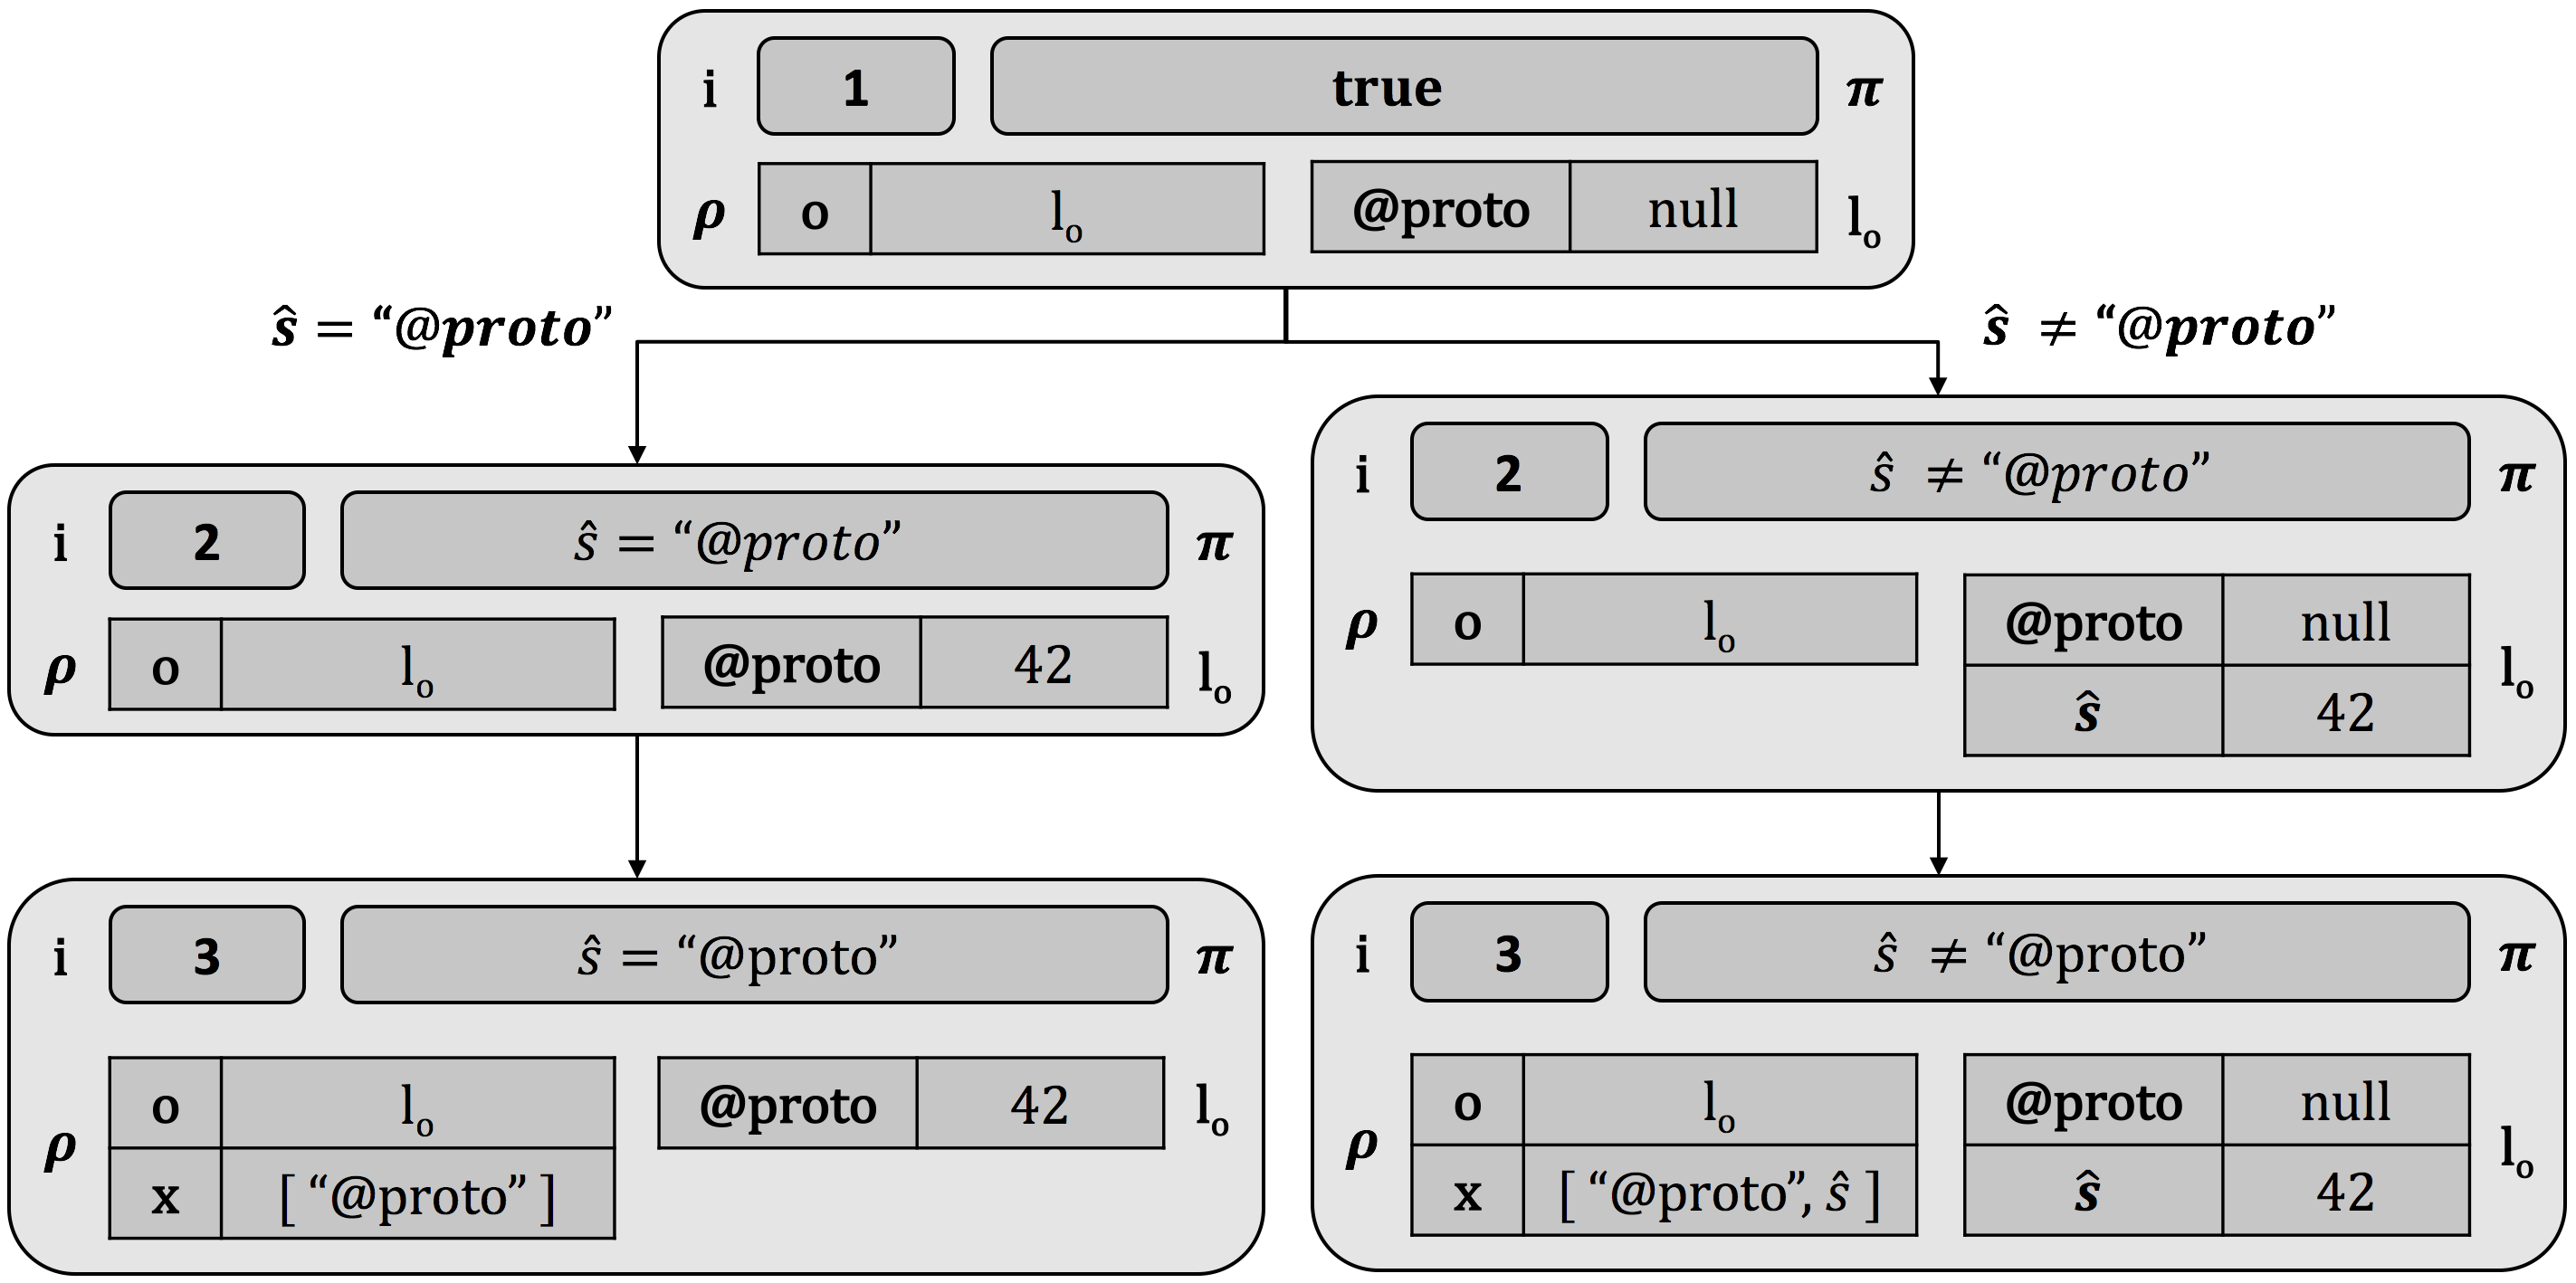
\includegraphics[width=0.83\textwidth]{symbSemEx.png}
\vspace*{-0.2cm}
\caption{Example of a \jilette symbolic execution}
\label{fig:sexecexample}
\vspace*{-0.5cm}
\end{figure*}

The next command to be executed is the property assignment $\mathtt{o[\hat{s}] := 42}$. In the symbolic semantics, there are two potential \textsc{Property Assignment} rules (\textsc{Found}, \textsc{Not Found}), and in our case, both of them are applicable. The key strategy is to branch on the targeted property of the object (in our case, the symbolic property $\hat{s}$ of object at location $\mathtt{l_o}$) being equal to any one or none of the already existing properties of the object (in our case, we have only $\mathtt{``@proto"}$), adding the appropriate equalities and inequalities to the path condition, and proceeding with the symbolic execution for all obtained branches. In this case, this means that the symbolic execution will branch on whether or not $\hat{s} = \mathtt{``@proto"}$. We obtain two symbolic states, shown in the second row of Figure \ref{fig:sexecexample}. The left branch corresponds to the (\textsc{Found}) case, when $\hat{s} = \mathtt{``@proto"}$: this equality is added to the path condition and the value of the property $\mathtt{``@proto"}$ is updated to 42. In the right branch, we have that $\hat{s} \neq \mathtt{``@proto"}$ (\textsc{Not Found}), hence object $\mathtt{o}$ has two properties: $ \mathtt{``@proto"}$, with value $\jsnull$; and $\hat{s}$, with value 42. 
The execution then continues in both branches with the property collection command $\mathtt{x := getFields(o)}$, which assigns the set of properties of the object $\mathtt{o}$ to variable~$\mathtt{x}$ (last row of Figure~\ref{fig:sexecexample}). Finally, we execute $\mathtt{assert\ (card \ x = 2)}$, asserting that the object $\mathtt{o}$ has exactly two properties, which we observe to hold in the right branch, but not in the left. Therefore, following the \textsc{Assert - False} rule, we obtain a failing symbolic execution trace, from which a concrete counter-model can be derived (that being: $\hat{s} = \mathtt{``@proto"}$).

\myparagraph{Transparency} 
Observe that a concrete state is also a symbolic state. Hence, we can feed a concrete state to the 
symbolic execution. In that case, the symbolic execution must behave exactly as the concrete 
execution. This is captured by the transparency theorem given below. 

\begin{theorem}[Transparency]\label{teo:transparency}
$\forall \, \heap, \heap', \store, \store', i, i', \ctx, \ctx', \, . \,$
\vspace{-5pt}
$$
  \semtranstrans{\heap, \store, i}{\heap', \store', i'}[\ctx][\ctx']
  \iff
  \symbtranstrans{\heap, \store, i, \jtrue}{\heap', \store', i', \jtrue}[\ctx][\ctx'] 
$$
\end{theorem}

\vspace{-5pt}
\myparagraph{Soundness} To establish the soundness of symbolic execution, we need to relate 
symbolic states to concrete states. To this end, we make use of \emph{symbolic environments} 
$\senv : \svars \rightharpoonup \vals$ mapping symbolic values to concrete values. 
A symbolic environment is said to be \emph{well-formed} if it maps symbolic 
values to concrete values of the appropriate type (e.g. symbolic strings are mapped to strings 
and symbolic numbers are mapped to numbers). In the following, we will always 
assume well-formed symbolic environments. 
%
Given a symbolic environment $\senv$, we define the interpretation of symbolic 
expressions, heaps, stores, and contexts as shown in Figure~\ref{fig:symbolic:interp}. 
We say that a symbolic environment is \emph{consistent} with a path condition 
$\pc$, written $\senv \vdash \pc$,  if and only if $\semexpr{\pc}{\senv} = \jtrue$. 
Given a symbolic state $(\sheap, \sstore, \sctx)$ and a path condition $\pc$, we define 
the models of the symbolic state under $\pc$, written $\smodels{\sheap, \sstore, \sctx}{\pc}$, 
as the set of concrete states that can be obtained from $(\sheap, \sstore, \sctx)$ using 
logical environments that are consistent with $\pc$. Formally:

{\small \begin{align}
\smodels{\sheap, \sstore, \sctx}{\pc} = \left\{ (\heap, \store, \ctx) \mid \exists \senv \, . \,  \semexpr{(\sheap, \sstore, \sctx)}{\senv} = (\heap, \store, \ctx) \, \wedge \,  \senv \vdash \pc  \right\} \\
\smodels{\sheap, \sstore}{\pc} = \left\{ (\heap, \store) \mid \exists \senv \, . \,  \semexpr{\sheap}{\senv} = \heap \, \wedge \, \semexpr{\sstore}{\senv} = \store \, \wedge \,  \senv \vdash \pc  \right\}
\end{align}}

\begin{figure}[t!]
{\small
\begin{tabular}{l}
$\quad${\bf Interpretation of Symbolic Expressions:}  \\
$
\quad
\semexpr{\val}{\senv} \semeq \val
\quad 
\semexpr{\svar}{\senv} \semeq \senv(\svar)
\quad 
\semexpr{\unoper\ \sexpr}{\senv} \semeq \semop{\unoper} (\semexpr{\sexpr}{\senv})
\quad 
\semexpr{\sexpr_1 \binoper \sexpr_2}{\senv} \semeq \semop{\binoper}(\semexpr{\sexpr_1}{\senv}, \semexpr{\sexpr_2}{\senv}) 
$
\\[3pt]
$\quad${\bf Symbolic Heaps:}  \\
$
\quad
 \semexpr{\hemp}{\senv} \semeq \hemp
\quad
\semexpr{\hcell{\loc}{\sexpr_p}{\sexpr_v}}{\senv} \semeq  \hcell{\loc}{\semexpr{\sexpr_p}{\senv}}{\semexpr{\sexpr_v}{\senv}}
\quad
\semexpr{\sheap_1 \dunion \sheap_2}{\senv} \semeq  \semexpr{\sheap_1}{\senv} \dunion \semexpr{\sheap_2}{\senv}
$%
%%
%%
\\[3pt]
$\quad${\bf Symbolic Stores:}  
$
 \semexpr{\storeemp}{\senv} \semeq \storeemp
\quad 
 \semexpr{(\jvar: \sexpr) \dunion \sstore}{\senv} \semeq (\jvar: \semexpr{\sexpr}{\senv}) \dunion \semexpr{\sstore}{\senv}
$%
\\[3pt]
$\quad${\bf Symbolic Contexts:}  
$ \semexpr{\lstemp}{\senv} \semeq \lstemp
\quad 
 \semexpr{(\pid, \sstore, \jvar, i, j) \lstcons \sctx}{\senv} \semeq (\pid, \semexpr{\sstore}{\senv}, \jvar, i, j) \lstcons \semexpr{\sctx}{\senv}
$%

\\[3pt]
$\quad${\bf Symbolic States:}  $\semexpr{(\sheap, \sstore, \sctx)}{\senv} \semeq (\semexpr{\sheap}{\senv}, \semexpr{\sstore}{\senv}, \semexpr{\sctx}{\senv})$
\end{tabular}
}
\caption{Interpretation of symbolic expressions, heaps, stores, and contexts.\label{fig:symbolic:interp}}
\vspace{-0.5cm}
\end{figure}

The soundness theorem (Theorem~\ref{teo:soundness:jsil:symb:exe}) states that if we have a symbolic trace captured by 
$\symbtranstrans{\sheap, \sstore, i, \pc}{\sheap', \sstore', i', \pc'}[\sctx][\sctx']$ 
and a concrete state $(\heap, \store, \ctx)$ in the models of the initial symbolic state under 
the final path condition $\pc'$, then there is a concrete symbolic state $(\heap', \store', \ctx')$ 
in the models of the final symbolic state under $\pc'$ such that: 
$\semtranstrans{\heap, \store, i}{\heap', \store', i'}[\ctx][\ctx']$. 
 We use the final path condition $\pc'$ for both the models of the initial and final 
symbolic states because we only care about the initial concrete states for which 
the concrete execution will follow the same path as the symbolic execution. 
%
\begin{theorem}[Soundness]\label{teo:soundness:jsil:symb:exe}
$\forall \, \sheap, \sheap', \heap, \sstore, \sstore', \store, i, i', \sctx, \sctx', \ctx, \pc, \pc' \, . \,$
\vspace*{-0.65cm}
$$
\begin{array}{l}
  \\  
\quad \symbtranstrans{\sheap, \sstore, i, \pc}{\sheap', \sstore', i', \pc'}[\sctx][\sctx'] 
   \ \wedge \ 
      (\heap, \store, \ctx) \in \smodels{\sheap, \sstore, \sctx}{\pc'} \\ \quad \quad
      	 \ \Rightarrow \ \exists (\heap', \store', \ctx') \, . \, 
	 	 \semtranstrans{\heap, \store, i}{\heap', \store', i'}[\ctx][\ctx']
		\, \wedge \, 
		(\heap', \store', \ctx') \in \smodels{\sheap', \sstore', \sctx'}{\pc'}  
\end{array}
$$
\end{theorem}
%
The \emph{bug-finding} corollary (Corollary~\ref{bug:finding}) states that if 
we find a symbolic trace that results in a failed assertion, 
then there also exists a concrete execution that will cause that assertion to fail.
Observe that the analysis is designed in such a way that there are no false positives, 
meaning that if we find a failing symbolic trace,
we can always instantiate its symbolic values obtaining a concrete counter-model for the 
failing assertion. This is essential, as \jilette is meant to be a \emph{bug-finding} tool.
%
\begin{corollary}[Bug-finding]\label{bug:finding}
$\forall \, \sheap, \sstore, \sctx, i, \pc, \pc' \, . \,$
\vspace*{-0.2cm}
$$
\begin{array}{l}
 \quad \symbtranstranserr{\sheap, \sstore, i, \pc}{\sctx}{\pc'} \implies 
     \exists \heap, \store, \ctx \, . \, \semtranstranserr{\heap, \store, i}[\ctx]
\end{array}
$$
\end{corollary}
%
Finally, the \emph{verification} corollary (Corollary~\ref{corollary:verification})
states that if we have symbolically explored all the possible execution paths
starting from a given symbolic state $(\sheap, \sstore, \sctx)$,  
then the execution of the program starting from  any concrete state in the models 
of the initial symbolic state (under the initial path condition) will result in a final concrete state
in the models of one of the final symbolic states (under its associated path condition).  
As \jilette does not infer loop invariants, if a \jsil program contains loops that cannot be unrolled statically, we will never be in the case of the verification corollary. 

\begin{corollary}[Verification]\label{corollary:verification}
$\forall \, \sheap, \sheap_i|_{i=1}^n, \sstore, \sstore_i|_{i=1}^n, 
\sctx, \sctx_i|_{i=1}^n, i, j_i|_{i=1}^n, \pc, \pc_i|_{i=1}^n \, . \,$
\vspace{-0.25cm}
$$
\begin{array}{l}
  \ \symbtranstrans{\sheap, \sstore, i, \pc}{\sheap_k, \sstore_k, j_k, \pc_k}[\sctx][\sctx_k]\mid_{k = 1}^n
      \ \wedge \ \pc \vdash \bigvee_{k=1}^n \pc_k \\ 
      \quad \implies 
         \forall \heap, \store, \ctx \, . \, (\heap, \store, \ctx) \in \smodels{\sheap, \sstore, \sctx}{\pc} \\
          \ \quad \implies \exists \heap', \store', \ctx', k\, . \, 
                  \semtranstrans{\heap, \store, i}{\heap', \store', j_k}[\ctx][\ctx'] \ \wedge \ 
                  (\heap', \store', \ctx') \in \smodels{\sheap_k, \sstore_k, \sctx_k}{\pc_k}
\end{array}   
$$ 
\end{corollary}
%
The {\bf proofs} of the above results are given in the Appendix. 


\subsection{Implementation}
\label{subsec:jsil:analysis:implementation}

Implementing a symbolic execution engine for \jsil is a non-trivial 
task, requiring a substantial engineering effort. 
% 
% 
Hence, instead of implementing the symbolic semantics of \jsil from scratch, we leverage on 
\rosette~\cite{Rosette1,Rosette2}, a symbolic virtual machine designed to 
enable swift development of new 
solver-aided languages. 
%
\rosette is a small extension of Racket~\cite{racket} equipped with a symbolic compiler with support 
for symbolic values and first order assertions. Because \rosette is itself solver-aided, languages 
implemented in \rosette can also make use of the solver-aided facilities provided by \rosette. 
Hence, by implementing a \emph{concrete} \jsil interpreter in \rosette, we obtain \emph{for free} a symbolic 
interpreter for \jsil. %consistent with the symbolic semantics described in  \S\ref{subsec:jsil:analysis:formalism}. 
%The idea of turning a concrete interpreter into a symbolic interpreter by embedding it in 
%
The implementation of the concrete interpreter in \rosette must fulfil the following criteria:
\begin{itemize}          
   \item \emph{Efficiency:} the implementation must promote \rosette's efficient behaviour;
   
   \item \emph{Termination:} the user must be given a way to establish a bound for the symbolic execution 
            of programs that loop on symbolic values; 
  
   \item \emph{Adequacy:} the symbolic execution of the concrete interpreter in \rosette 
            must be consistent with the symbolic semantics described in \S\ref{subsec:jsil:analysis:formalism}. 
\end{itemize}

%- describe the \rosette approach to the implementation of symbolic analysis 
% - describe the encoding of \jsil concrete/symbolic states in \rosette 
% - explain the \jsil interpreter implemented in \rosette and its connection to the \jsil concrete semantics  and symbolic semantics 
%- give snippets of the interpreter 
%- discuss implementation strategies that enable \rosette to work properly

\myparagraph{Implementing \jsil in \rosette}
We first show
how to model the concrete \jsil state. Below are our \rosette encodings of \jsil heaps, stores, 
and call stacks. 
Heaps are modelled as pairs of locations and lists of property-value pairs, 
stores as lists of variable-value pairs, and call stacks as lists of lists, each of which
contains the \rosette encoding of the appropriate four elements. 
\jsil variables and function identifiers are modelled 
as Racket symbols.\footnote{Racket symbols are uninterpreted values and can be viewed as immutable strings.} 
\jsil values with \rosette correspondents are mapped accordingly; the remaining 
ones are modelled as Racket symbols (e.g. \jsil types, $\jsundefined$, $\jsnull$, and $\jsilempty$). 

\begin{display}{\rosette implementation of \jsil symbolic state}
{\scriptsize
\begin{mathpar}
\inferrule[\textsc{Empty Heap}]
  {}{\roscomp{\hemp} \semeq (\racketlist)} 
\and 
\inferrule[\textsc{Non-empty Heap}]
  {
  	 \sheap_1 = \big((l, \sexprp_i) \mapsto \sexprv_i\big)\mid_{i = 0}^n   
	 \quad 
	 (\loc, -) \not\in \domain(\sheap_2)
  }{\roscomp{\sheap_1 \dunion \sheap_2} \semeq  (\racketcons (\racketcons \loc \, (\racketlist \, (\racketcons \sexprp_0 \, \sexprv_0) \cdots   (\racketcons \sexprp_n \, \sexprv_n)))  \ \roscomp{\sheap_2})} 
 \\
\inferrule[\textsc{Empty Store}]
  {}{\roscomp{\storeemp} \semeq (\racketlist)} 
\and 
\inferrule[\textsc{Non-Empty Store}]
  {}{\roscomp{(\jvar: \sexpr) \dunion \sstore} \semeq (\racketcons \, (\racketcons \, (\racketquote \jvar) \ \sexpr) \,  \roscomp{\sstore})} 
\\ 
\inferrule[\textsc{Empty Context}]
  {}{\roscomp{\lstemp} \semeq (\racketlist)} 
\quad 
\inferrule[\textsc{Non-Empty Context}]
  {}{\roscomp{(\fid, \sstore, \jvar, i, j) \lstcons \sctx} \semeq  (\racketcons \,  (\racketlist \, (\racketquote \fid) \, \roscomp{\sstore} \, (\racketquote \jvar) \, i \, j) \, \roscomp{\sctx})} 
\end{mathpar}}
\end{display}

The implementation of \jsil commands precisely follows their concrete semantics as 
described in \S\ref{subsec:jsil:analysis:formalism}. 
To show this, let us consider the fragment of the \jsil interpreter that implements 
the \prooflab{Property Assignment} rule, shown in Figure~\ref{rosette:interpreter:fragment}.
The figure shows three functions: \dtag{1} \schemeinline|(run-bcmd bcmd heap store)|, for 
executing basic commands, \dtag{2} \schemeinline|(update-heap heap loc prop val)|, for 
updating the heap \schemeinline|heap| by setting the value of the 
the property \schemeinline|prop| of the object denoted by \schemeinline|loc| to \schemeinline|val|, 
and \dtag{3} \schemeinline|(update-pv-list pv-list prop new-val)|,
for updating the property-value list \schemeinline|pv-list| by setting \schemeinline|prop|
to \schemeinline|new-val|. 

\lstset{language=Scheme, numbers = left}

\begin{figure}[t!]
\centering
\begin{lstlisting}
(define (run-bcmd bcmd heap store)
  (let ((cmd-type (first bcmd)))
    (cond
    	[(eq? cmd-type 'p-assign)
      	 (let* ((loc-val  (run-expr (second bcmd) store))
                (prop-val (run-expr (third bcmd)  store))
                (rhs-val  (run-expr (fourth bcmd) store)))
            (cons (update-heap heap loc-val prop-val rhs-val) store))]
         ...)))
\end{lstlisting}

\begin{lstlisting}
(define (update-heap heap loc prop val)
  (cond
    [(null? heap) (error "Inexistent object")]
    [(equal? (caar heap) loc)
     (cons (cons loc (update-pv-list (cdar heap) prop val)) (cdr heap))]
    [ else (cons (car heap) (update-heap (cdr heap) loc prop val))]))
\end{lstlisting}

\begin{lstlisting}         
(define (update-pv-list pv-list prop new-val)
  (cond
    [(null? pv-list)
     (list (cons prop new-val))]
    [(equal? (caar pv-list) prop)
     (cons (cons prop new-val) (cdr pv-list))]
    [ else (cons (car pv-list) 
              (update-pv-list (cdr pv-list) prop new-val))]))
\end{lstlisting}
\vspace*{-0.3cm}
\caption{Fragment of the \jsil Interpreter in \rosette\label{rosette:interpreter:fragment}}
\vspace*{-0.5cm}
\end{figure}

\jsil commands are represented in \rosette as \emph{s-expressions}. 
 For instance, the property assignment basic command $[\jsilexpr_1, \jsilexpr_2] := \jsilexpr_3$
 is represented as: 

\vspace*{-0.2cm}
{\small $$
\mathtt{(list \ (quote\ {p\text{--}assign}) \ \roscomp{\jsilexpr_1} \ \roscomp{\jsilexpr_2} \ \roscomp{\jsilexpr_3})}
$$}
\vspace*{-0.4cm}

\noindent Therefore, the interpreter of basic commands first checks if the first element of the 
list representing the command is equal to \schemeinline|p-assign|. If it is, 
it uses the function \schemeinline|run-expr| to evaluate the three \jsil expressions 
comprising the property-assignment in the appropriate order. Then, it invokes the 
function \schemeinline|update-heap| to perform the actual update. 
The function \schemeinline|update-heap| recursively iterates over all heap objects
to find the object whose property is to be updated and, when it finds it, 
uses the function \schemeinline|update-pv-list| to update the corresponding 
field-value list. If it does not find it, it will raise an error. However, due to the concrete semantics of \jsil, this case is never triggered.

\lstset{language=Scheme, numbers=none, backgroundcolor=\color{mygray}}
\myparagraph{Efficiency}
It is often possible for more than one transition of the symbolic 
semantics to be applicable during symbolic execution, likely 
giving rise to an intractable number of possible symbolic states. 
To counter this problem, \rosette makes use of a sophisticated 
symbolic state merging algorithm, which factors out the common 
part between multiple symbolic states  in order to expose more 
opportunities for concrete evaluation. The portions of the state 
that are not mergeable are represented as \emph{guarded symbolic unions}. 
Our goal is to write the interpreter code in a way that helps 
\rosette merge sets of possible symbolic states, yielding minimal 
guarded symbolic unions.
To illustrate this point, let us consider the symbolic execution 
of the property assignment $\mathtt{o[\hat{s}] := 42}$ in the 
symbolic heap represented in \rosette as follows: 
%
\begin{lstlisting}
(lo (("@proto" null) ("a" 0) ("b" 1)))
\end{lstlisting}
%
with a symbolic store mapping \schemeinline|o| to \schemeinline|lo| and 
the path condition {\small $\mathtt{\hat{s} = \text{\texttt{"a"}} \ \vee \hat{s} = \text{\texttt{"b"}}}$}.
The two resulting symbolic heaps are represented in \rosette as :  
%
\begin{lstlisting}
(lo (("@proto" null) ("a" (? (= s "a") 42 0)) ("b" (? (= s "b") 42 1)))
\end{lstlisting}
%
One can see that \rosette manages to push the guarded unions to 
the object cells that may be affected by the property assignment, maintaining a common 
property-value list for both resulting symbolic states. 
%
Now, let us change the code of line 6 of \schemeinline|update-pv-list| 
(in Figure~\ref{rosette:interpreter:fragment}) to:  
\begin{lstlisting}
(append (cdr pv-list) (cons prop new-val))
\end{lstlisting}
This change in the interpreter makes the order of the cells in the property-value 
list change depending on which property gets updated. 
Now, \rosette needs to create a single guarded union 
with the two possible resulting property-value lists: 
\begin{lstlisting}
(lo (? (= s "a") 
       (("@proto" null) ("b"  1) ("a" 42)) 
       (("@proto" null) ("a"  0) ("b" 42))))
\end{lstlisting}

\myparagraph{Termination} The \jsil symbolic execution engine does not 
include the abstraction mechanisms which would allow it to finitise the symbolic 
execution of loops depending on symbolic values~\cite{abstract:symbolic:exec}. 
Hence, the user is asked to specify an upper bound on the number of times
the symbolic execution is allowed to branch on symbolic values by using
conditional gotos. 
Once that upper bound is reached, if a conditional goto that branches 
on a symbolic value is encountered, the symbolic execution stops.  


\myparagraph{Adequacy} 
We strongly believe that the symbolic execution of the concrete interpreter 
in \rosette is consistent with respect to the \jsil symbolic semantics. 
In fact, we have ``reverse-engineered'' our \jsil symbolic execution by 
observing in detail the guarded unions produced by Rosette for each of 
the \jsil commands. Due to its complexity and scale, 
{a formal proof would require
mechanisation}, which is, unfortunately, beyond our manpower.
 
%Hence, the user is asked to specify an upper bound on the number of times
%the symbolic execution is allowed to branch depending on symbolic values. 
%Once that upper bound is reached, if a conditional goto that branches 
%on a symbolic value is encountered, the symbolic execution simply stops.  

\lstset{backgroundcolor=\color{white}}

\section{Symbolic Testing for JavaScript}
\label{sec:sym:exec:js}

\begin{figure}[t]
\centering
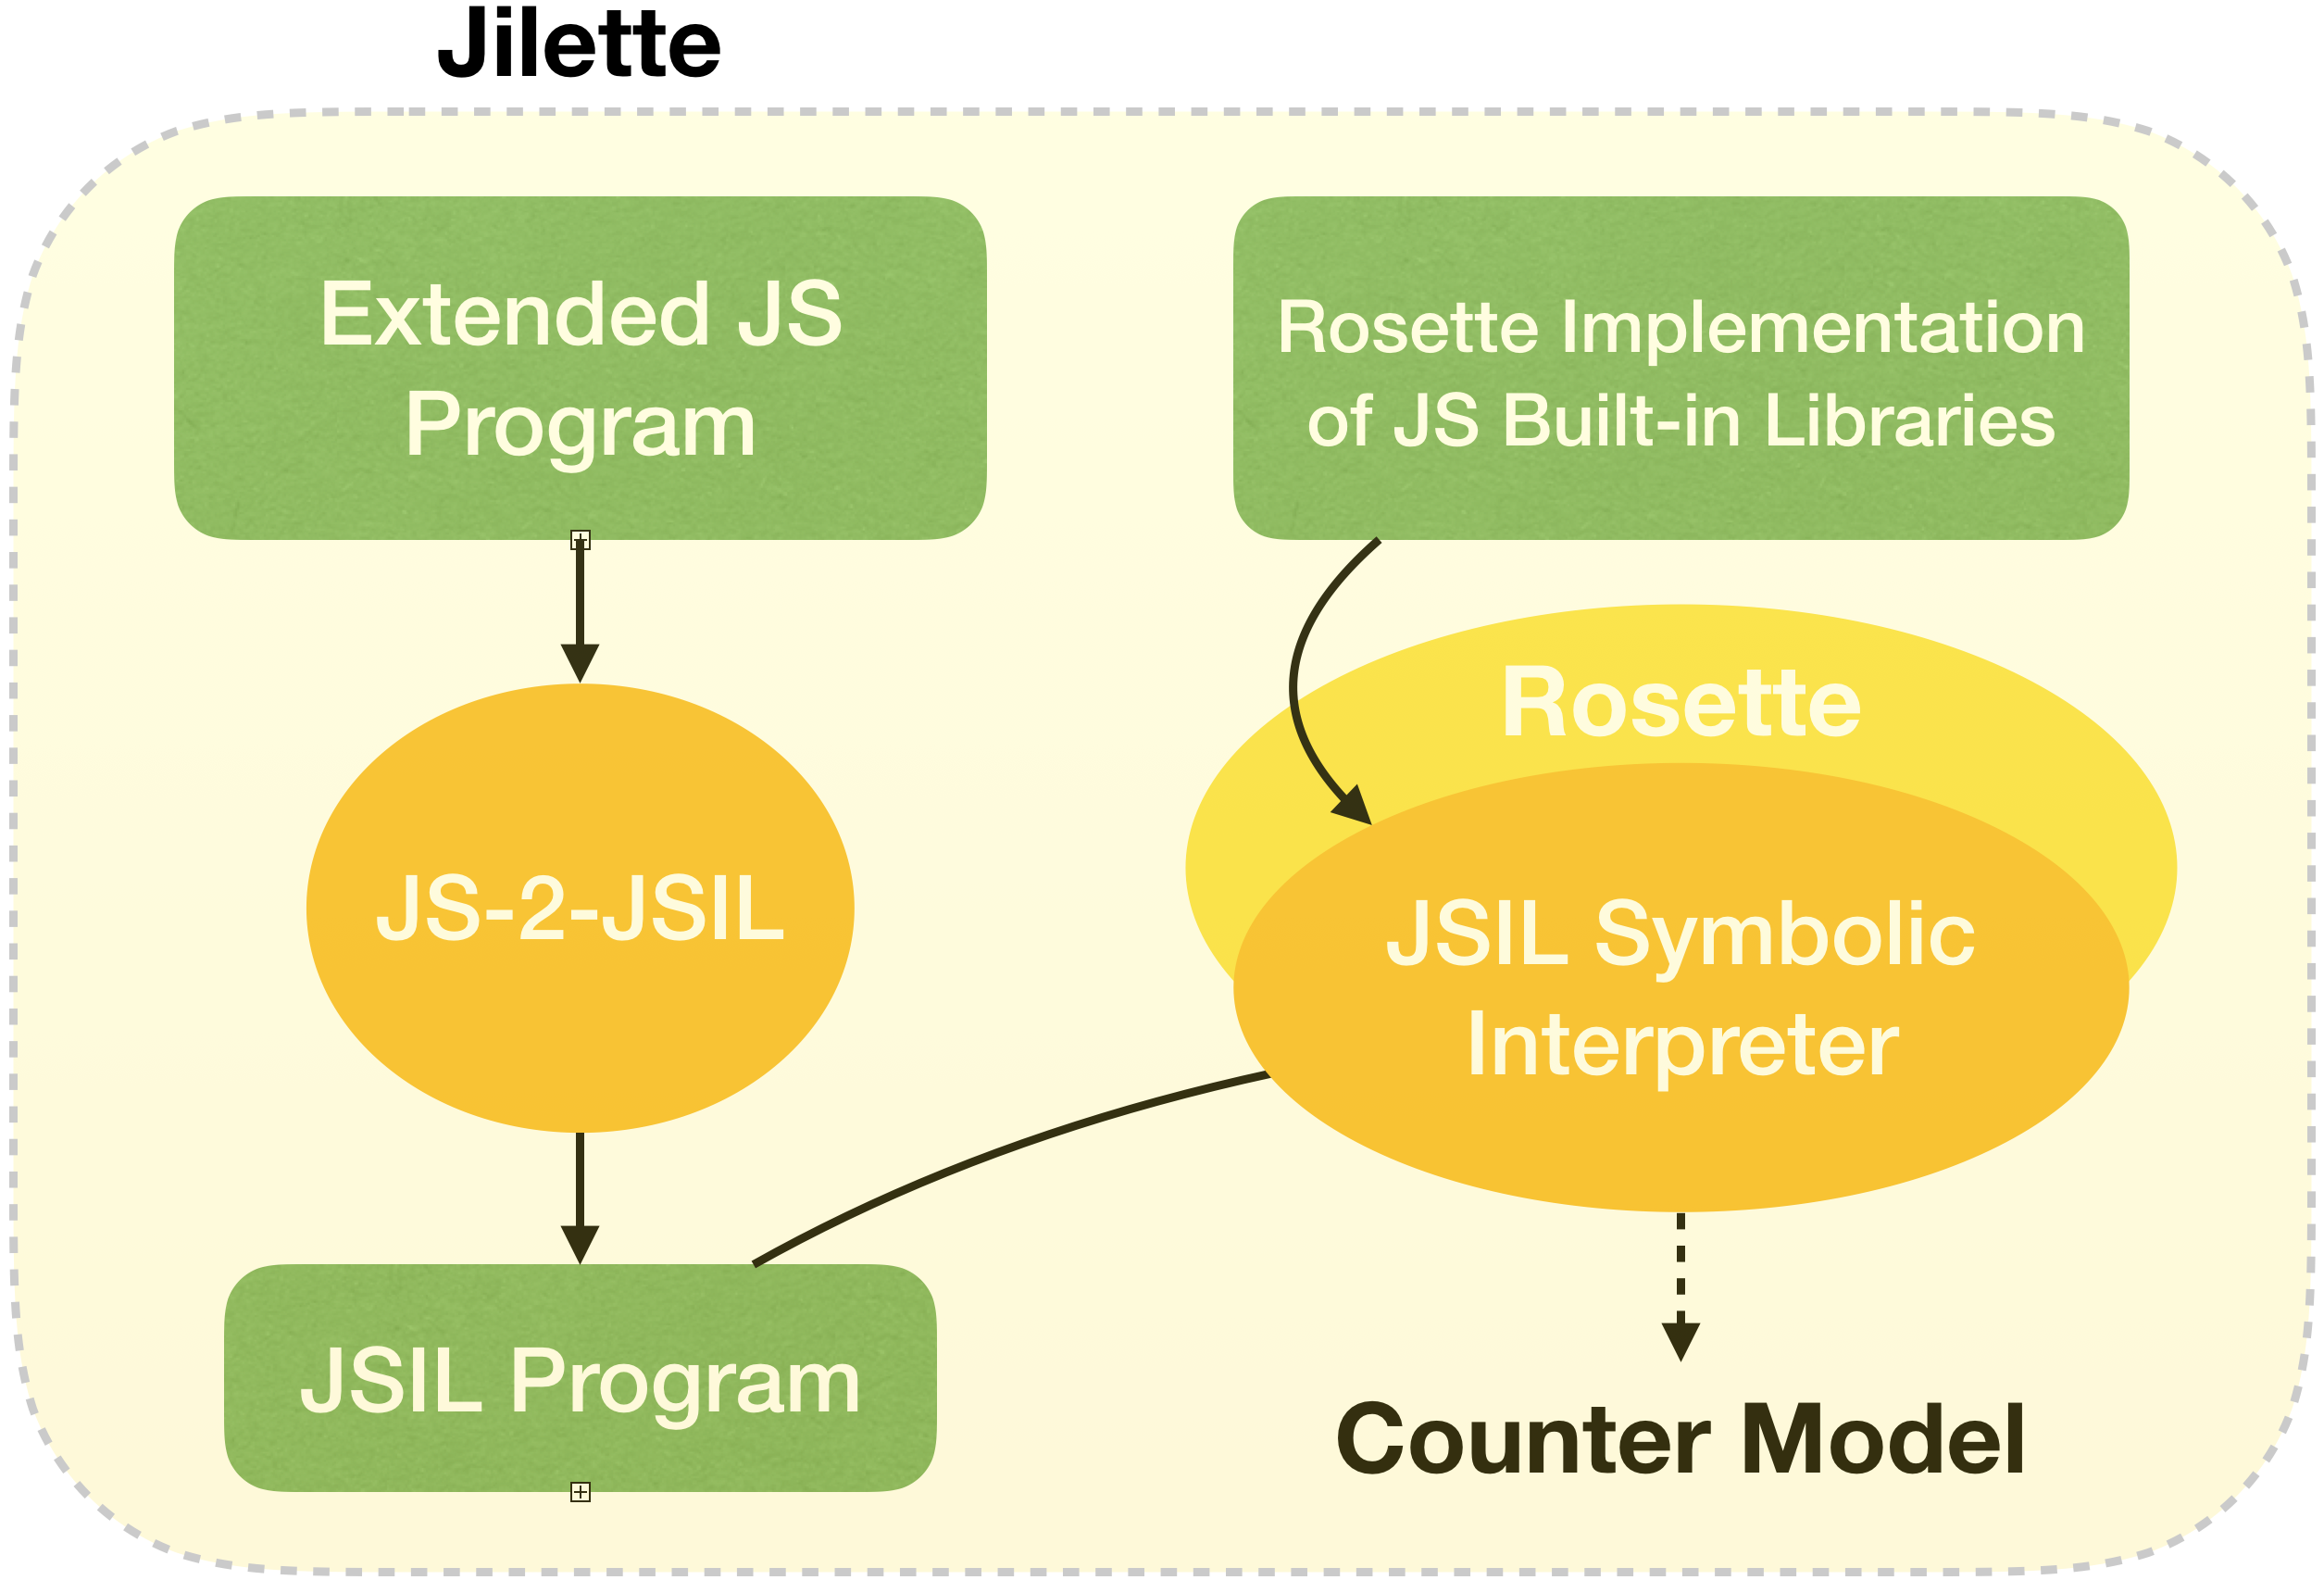
\includegraphics[width=0.7\textwidth]{figures/jilette.png}
\vspace*{-0.2cm}
\caption{\jilette: Symbolic execution for JavaScript}
\vspace*{-0.3cm}
\label{fig:jilette:diagram}
\end{figure}

Symbolic execution designed directly on JavaScript is not feasible, for the same reasons verification is not~\cite{JoseCADE}: the semantics of the language is too complex, with numerous intertwined internal functions called under the hood. In particular, the simple assignment alone would have more than twenty potential branchings. Our approach is to symbolically analyse JavaScript code by first compiling it to \jsil, using~\JSComp~\cite{javert}, and then feeding the compiled \jsil code to our \jsil symbolic interpreter, described in \S\ref{sec:jsil:symb:exec}.

In \S\ref{symb:exec:comp}, we explain how we enable symbolic execution for JavaScript using \JSComp and Rosette, by extending the language with new constructs for the creation of symbolic values and the checking of assertions.
In \S\ref{symbolic:testing}, we explain how this symbolic execution can be used for the symbolic testing of JavaScript code. 
Finally, in \S\ref{builtins}, we conclude with the presentation 
of a general approach for handling the symbolic execution of JavaScript built-in libraries.
More concretely, it is possible to extend the \jsil symbolic interpreter with \rosette implementations of JavaScript built-in libraries in a streamlined manner.  
These implementations are both an easy way to get a better coverage of the standard and 
match the abstraction level of the generated JSIL code precisely with the abstraction level 
of Rosette, maximising the use of Rosette's native solver-aided facilities.

%to make sure that we make proper use of theof \rosette.    

\subsection{Symbolic Execution by Compilation} 
\label{symb:exec:comp}

\myparagraph{Extending JavaScript Syntax}
We extend the syntax of JavaScript with special logical expressions $\jslexpr$, 
and the following constructs: %(corresponding to JavaScript normal expressions): 
\dtag{1} $\jsassert(\jslexpr)$, stating that whenever the \emph{assert} is reached, 
the logical expression $\jslexpr$ must evaluate to $\jtrue$; 
\dtag{2} $\jsassume(\jslexpr)$, stating that we \emph{assume} $\jslexpr$ to hold along the
current program path; 
\dtag{3} $\jssymbstring()$, for creating a fresh symbolic string; and
\dtag{4} $\jssymbnumber()$, for creating a fresh symbolic number. 
The \emph{assert} and \emph{assume} constructs expect as an argument 
a logical expression. 
Logical expressions $\jslexpr$ are given by the grammar 
$\jslexpr \triangleq \jslit \mid \jsvar \mid \unoper\ \jslexpr \mid \jslexpr \binoper \jslexpr$, 
where $\jslit$ ranges over JavaScript literal values (numbers, booleans, strings, \jsinline|undefined|, and \jsinline|null|), $\jsvar$ over JavaScript variables, 
$\unoper$ over the \jsil unary operators, and $\binoper$ over the \jsil binary operators.
Note that the JavaScript binary and unary operators may have side effects; furthermore,  
the semantics of these operators often includes several implicit type coercions 
performed in a specific (and counter-intuitive) order. 
Hence, we do not allow arbitrary JavaScript expressions (using JavaScript 
binary and unary operators) as the arguments for the \emph{assume} and 
the \emph{assert} constructs. Instead, we use the \jsil unary and binary operators, which have a very clear and simple semantics, without coercions or side-effects.

\myparagraph{Extending \JSComp}
Instead of giving a formal semantics for the newly introduced constructs, we explain 
their meaning by showing their compilation to \jsil. 
Importantly, the JavaScript variable store is emulated in the heap. 
Hence, a JavaScript variable $\jsvar$ is not compiled to a \jsil variable $\jvar$, but to a sequence  
of \jsil commands for retrieving the value of $\jsvar$ from the heap cell in which it is stored. 
A full description of \JSComp is out of the scope of this paper; see~\cite{Daiva2017}
for further details.
%
In the following, we will assume given a function $\compile : \jstmts \rightharpoonup \lists(\cmds) * \jvars$ mapping JavaScript expressions 
and statements to lists of \jsil commands paired up with \jsil variables. 
In a nutshell, $\compile(\jstmt) = ([ \jcmd_1, ..., \jcmd_n], \jvar)$ means that the compilation 
of the JavaScript statement $\jstmt$ results in the list of \jsil commands $[ \jcmd_1, ..., \jcmd_n]$, 
and that after the execution of these commands, the value to which $\jstmt$ evaluates in the 
JavaScript semantics is stored in the \jsil variable $\jvar$. 
%
Below we show the extension of $\compile$ for the constructs introduced above. 
The definition of $\compile$ relies on an auxiliary compiler $\compilel : \jlexprs \rightharpoonup \lists(\cmds) * \exprs$, 
for translating JavaScript logical expressions.

\begin{display}{Extension $\compile : \jstmts \rightharpoonup \lists(\cmds) * \jvars$ and $\compilel : \jlexprs \rightharpoonup \lists(\cmds) * \exprs$}
{\scriptsize
\begin{mathpar}
\inferrule[\textsc{Assume}]
  {
     \compilel(\jslexpr) = [\jcmd_1, ..., \jcmd_n], \jsilexpr
     \and 
     \jvar' \text{ fresh} 
     \\\\ 
     \jcmd_{n+1} = \jvar' := \jsilempty 
     \quad
     \jcmd_{n+2} = \assume(\jsilexpr) 
  }{\compile(\jsassume(\jslexpr)) \semeq [\jcmd_1, ..., \jcmd_n, \jcmd_{n+1}, \jcmd_{n+2}], \jvar'} 
\and
\inferrule[\textsc{Assert}]
  {
     \compilel(\jslexpr) = [\jcmd_1, ..., \jcmd_n], \jsilexpr
     \and 
     \jvar' \text{ fresh} 
     \\\\ 
     \jcmd_{n+1} = \jvar' := \jsilempty 
     \quad
     \jcmd_{n+2} = \assert(\jsilexpr) 
  }{\compile(\jsassert(\jslexpr)) \semeq [\jcmd_1, ..., \jcmd_n, \jcmd_{n+1}, \jcmd_{n+2}], \jvar'}
  %
  \\
  %
  \inferrule[\textsc{Symbolic String}]
  {
    \sstring \text{ fresh} 
    \and 
    \jvar \text{ fresh}
  }{\compile(\jssymbstring()) \semeq [ \jvar := \sstring ], \jvar}   
  %
  \and
  %
  \inferrule[\textsc{Symbolic Number}]
  {
    \snumber \text{ fresh} 
    \and 
    \jvar \text{ fresh}
  }{\compile(\jssymbnumber()) \semeq [ \jvar := \snumber ], \jvar}    
   %
  \and
  %
  \inferrule[\textsc{Literal}]
  {}{\compilel(\jslit) \semeq [], \jslit}   
  %
 \and
  %
  \inferrule[\textsc{JS Var}]
  {
     \compile(\jsvar) = [ \jcmd_1, ..., \jcmd_n ], \jvar
  }{\compilel(\jsvar) \semeq [ \jcmd_1, ..., \jcmd_n ], \jvar }    
   %
  \\
  %
  \inferrule[\textsc{Unary Operator}]
  {
     \compilel(\jslexpr) = [ \jcmd_1, ..., \jcmd_n ], \jvar
  }{\compilel(\unoper\ \jslexpr) \semeq [ \jcmd_1, ..., \jcmd_n ], \unoper\ \jvar }     
   %
  \and
  %
  \inferrule[\textsc{Binary Operator}]
  {
     \compilel(\jslexpr_1) = [ \jcmd_1, ..., \jcmd_n ], \jvar_1 
     \quad
     \compilel(\jslexpr_2) = [ \jcmd_1', ..., \jcmd_n'], \jvar_2
  }{\compilel(\jslexpr \binoper \jslexpr) \semeq [ \jcmd_1, ..., \jcmd_n, \jcmd_1', ..., \jcmd_n' ], \jvar_1\binoper \jvar_2 }     
\end{mathpar}}
\end{display}



\subsection{Symbolic Testing by Example} 
\label{symbolic:testing}

\lstnewenvironment{lstjsex}{\lstset{language=JavaScript,basicstyle=\fontsize{8}{8}\ttfamily,escapeinside={~}{~}, numbers=none, backgroundcolor=\color{mygray}}}{}


We illustrate how \jilette is used to write symbolic tests for JavaScript code by using the JavaScript implementation 
of a  \emph{key-value map} given in Figure~\ref{map:example}~(left). 
This implementation contains four functions: 
\jsinline|Map|, for constructing an empty map;
\jsinline|get|, for retrieving the value associated with the key given as input;
\jsinline|put|, for inserting a new \emph{key-value pair} into the map and updating the values associated with existing keys; and
\jsinline|validKey|, for deciding whether a key is valid.

\myparagraph{Prototype chains and $\mathtt{Object.prototype}$}
In order to better understand the implementation of the map library as well as its possible bugs, 
one must first understand the \emph{prototype-based inheritance} mechanism of JavaScript. 
Every JavaScript object has a prototype, which (for presentation purposes) we assume to 
be stored  in an internal property \jsinline|@proto|. In order to determine the value of a property
\jsinline|p| of an object \jsinline|o|, the semantics first checks if \jsinline|o| has a 
property named \jsinline|p|, in which case the property look-up yields its value. Otherwise, the 
semantics checks if \jsinline|p| belongs to the properties of the prototype of \jsinline|o| and so 
forth. Hence, in the example, when looking up the value of the property \jsinline|hasOwnProperty|
of the object \jsinline|contents|, one gets the value associated with the property  \jsinline|hasOwnProperty|
of its prototype.
The sequence of objects that can be accessed from a given object through the inspection 
of the respective prototypes is called a \emph{prototype chain}.
Prototype chains typically finish with the object \jsinline|Object.prototype| from which JavaScript 
programs can access a number of built-in functions, which are part of the language runtime environment and are used for inspecting and manipulating objects.
An example of such a function is \jsinline|hasOwnProperty(p)|, which checks whether or not the object 
on which it is invoked has the property \jsinline|p| (e.g. {\small \jsinline|map.hasOwnProperty("_contents")|}
evaluates to \jsinline|true| when evaluated in the heap shown in Fig.~\ref{map:example}-(right), 
because the object \jsinline|map| has a property named~\jsinline|"_contents"|). 

 \begin{figure}[t!]
 \begin{minipage}{0.56\textwidth}
 \begin{lstjs}[firstnumber=1]
function Map () { this._contents = {} }

Map.prototype.get = function (k) {
  var c = this._contents;
  if (c.hasOwnProperty(k)) {
    return this._contents[k] 
  } else { return null }
}

Map.prototype.put = function (k, v) {
  var c = this._contents;
  if this._contents.validKey(k)) {  
    contents[k] = v   
  } else
    throw new Error("Invalid Key");
} 

Map.prototype.validKey = function (k) { ... }
\end{lstjs}
\end{minipage}
\ 
 \begin{minipage}{0.43\textwidth}
 \vspace*{-0.3cm}
 \hspace*{-1.2cm}
 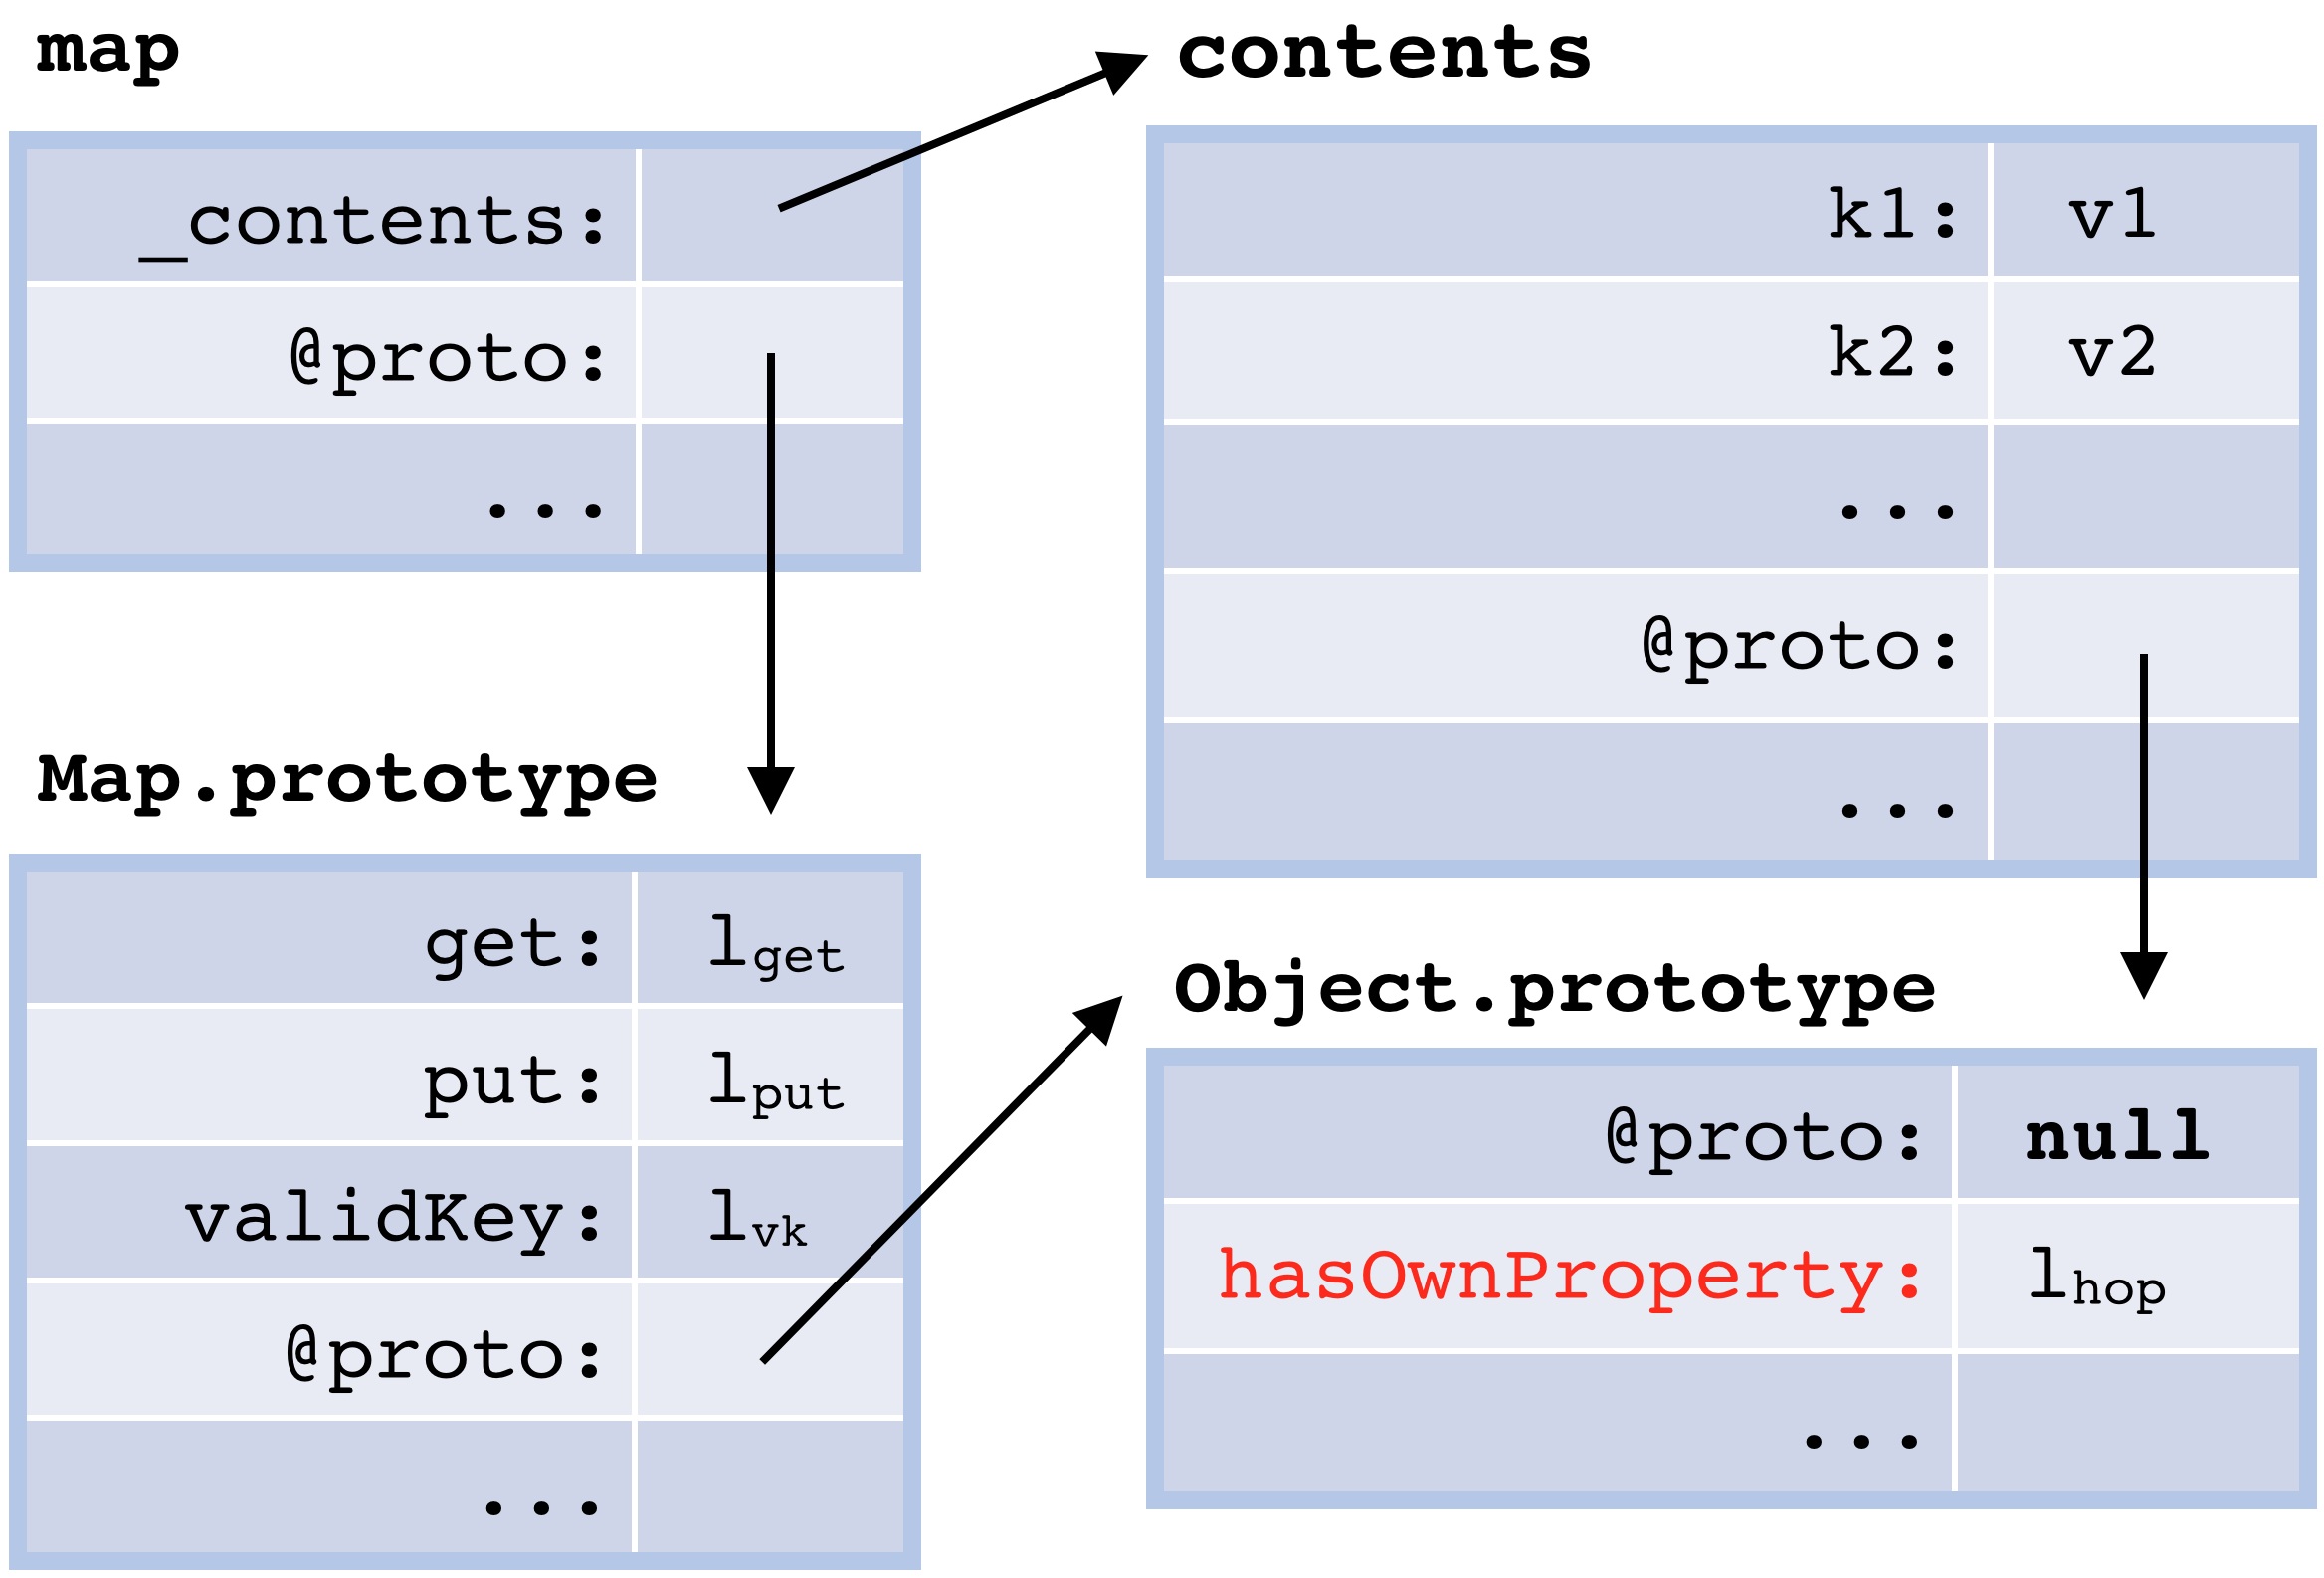
\includegraphics[width=1.2\textwidth]{figures/mapDiagram.png}
 \end{minipage}
\vspace*{-0.3cm}
\caption{JS map implementation (left) and example of a map library heap (right) \label{map:example}}
\end{figure}

\myparagraph{Bug-finding}
The map library implements a \emph{key-value map} as an object with property \jsinline|_contents|, denoting the object used to store the map contents.  
The named properties of \jsinline|_contents| and their value attributes correspond to the map keys and values, respectively.
As the functions \jsinline|get|, \jsinline|put|, and \jsinline|validKey| are to be shared between all map 
objects, they are defined as properties of \jsinline|Map.prototype|, which is the prototype 
of the objects that are created using \jsinline|Map| as a constructor (e.g.~using~\jsinline|new Map()|). 
%
Note that one can insert a key-value pair with \jsinline|"hasOwnProperty"| as a key into the map. 
By doing this, \jsinline|"hasOwnProperty"| in the prototype chain of
\jsinline|_contents| is overridden and subsequent calls to \jsinline|get| will fail. 
Consider the following symbolic test:
\begin{lstjsex}
var s1 = __s(); var n1 = __n(); 
var m = new Map();  m.put(s1, n1); var r = m.get(s1);  
assert(n1 = r)
\end{lstjsex}
%
The symbolic test above checks for a desired property of the library---if we were to put a key/value pair \jsinline|(k, v)| into the map, then we should be able to retrieve the value \jsinline|v| using the key \jsinline|k|. We can run \jilette on this test to reveal the bug discusses above. Indeed, \jilette generates
the failing model: \jsinline|s1 = "hasOwnProperty"|. 

This example also highlights how \jilette is approachable, does not require 
specialist knowledge, and can, therefore, be used by almost any JavaScript developer. 
The annotation burden amounts to the creation of symbolic variables and the writing of assertions, remaining minimal and intuitive, in stark contrast with the standard annotation 
burden of verification tools.

%- Extensible Interpreter 
% - an easy way to have more coverage 
% - match the abstraction level of the generated code to the abstraction level of \rosette 

\subsection{Supporting JavaScript Built-in Libraries}
\label{builtins}

JavaScript comes equipped with a rich runtime environment (described in Chapter 15 of the 
ES5 standard~\cite{ecma}), which consists of \emph{built-in libraries} that support advanced manipulation of, for example, objects, arrays, strings, regular expressions, and dates, among others. 
In this section, we identify two important challenges related to supporting the symbolic execution of
JavaScript programs that interact with built-in libraries and explain how we solve them in \jilette. 

\JSComp models built-in library functions as \jsil procedures, which can be called from within the compiled JavaScript code. However, the current runtime environment of \JSComp does not support all built-in libraries described in the standard. In particular, it doesn't support regular expressions, parts of the String library that use regular expressions, parts of the Date library, and JSON objects. The partiality of \JSComp when it comes to supporting JavaScript built-in libraries 
gives rise to the first challenge:  
\begin{quote}
\emph{Challenge 1:} \jilette should allow for modular addition of  
implementations of built-in libraries not yet covered by \JSComp.  
\end{quote}

Most JavaScript library functions are described in the language standard in terms of 
more elementary operations. For instance, operations on strings are often described in terms 
of operations on the characters that comprise the string, and often involve loops (c.f. \jsinline|String.lastIndexOf|, Ch.15.5.4.8~\cite{ecma}).
The \jsil implementations of the JavaScript built-in libraries follow the standard line-by-line. 
This is meant to emphasise that the compiler does, in fact, fully adhere to the language standard. 
However, for some of these built-in library functions, direct \rosette correspondents exist. 
%
In such cases, we argue that these correspondents should be used instead of the 
functions provided by \JSComp, to minimise potential branching and looping on symbolic values. 
Hence, we state the second challenge as follows: 
\begin{quote}
\emph{Challenge 2:} \jilette should prioritise native \rosette operations
to the operations provided by \JSComp in the cases in which the native \rosette
operations and JavaScript operations exactly match.
\end{quote}

\myparagraph{\rosette models of JavaScript built-in functions}
To solve these two challenges, \jilette supports the on-the-fly extension of the \jsil interpreter 
with \rosette implementations of JavaScript built-in functions, which we call \rosette \emph{models}. 
Hence, every time the interpreter evaluates a procedure call, it first checks whether or 
not it corresponds to a built-in function for which there is a \rosette model. If it does, 
instead of executing the standard procedure call rule, the interpreter will instead 
execute the appropriate \rosette model. 

Below, we show a simplified \rosette model for \jsinline|String.prototype.replace|~(c.f. Ch.15.5.4.11~\cite{ecma}).
Observe that this model uses the natively supported function \schemeinline|string-replace|, 
thus taking advantage of \rosette reasoning capabilities.
This example illustrates an important point about the difference between JavaScript and
\rosette operations: \schemeinline|string-replace| works only with strings, but \jsinline|String.|\jsinline|prototype. |\jsinline|replace| can take arguments of any type that then get coerced to strings. Since \JSComp does not have an implementation of \jsinline|String.replace|, the \rosette model will report an error if it receives non-string arguments.
\lstset{language=Scheme, numbers=none, backgroundcolor=\color{mygray}}
\begin{lstlisting}
(define (replace str from to)
  (if (and (string? str) (string? from) (string? to))
      (list (quote normal) (string-replace str from to #:all? #f))
      (error "Unsupported call to String.prototype.replace")))
\end{lstlisting}

\myparagraph{Bug-finding with strings}
By using the appropriate \rosette models for string operations, \jilette can find bugs in  
non-trivial JavaScript programs that manipulate strings. For instance, consider 
the following naive JavaScript implementation of a string sanitiser meant to remove 
all occurrences of \emph{script tags} inside untrusted strings (for instance, those coming 
from user input or untrusted servers).
To this end, the programmer chooses to 
replace all occurrences of the string \jsinline|"script"| in the string given 
as input with \jsinline|"s"|. 
\begin{lstjsex}
function sanitise (str) { return str.replace("script", "s") }
\end{lstjsex}
Now, we can use \jilette to test if the sanitiser meets its purpose, that is, that all
strings, after being sanitised, do not contain the substring \jsinline|"script"|:
\begin{lstjsex}
var s = sanitise(__s()); 
var x = ! (s.contains("script")); d
assert(x) 
\end{lstjsex}
\jilette will, in fact, be able to come up with a counter-model for this assertion. Concretely, \jsinline|s1 = "scriptcript"|. Despite its simplicity, this example illustrates the complexities underpinning the 
design and implementation of robust string sanitisers, a commonly  
used defense mechanism against XSS attacks~\cite{song}. 
 
 

 
 

%Furthermore, the \jsil language itself does not feature regular expressions or native arrays, 
%and has very few operators on strings. 
%This means that, for instance, more advanced operations on strings (such as 
%\jsinline|lastIndexOf|) need to be implemented as loops over the characters that comprise 
%the string. 
%






